%%\documentclass[twoside,openright,a4paper,11pt]{book}
%%
%%
\usepackage[utf8]{inputenc}
\usepackage[francais]{babel}
\usepackage[T1]{fontenc}

\addto\captionsfrench{\def\tablename{\textsc{Tableau}}}% pour avoir TABLEAU et pas TABLE dans les légendes des tableaux

%%%%%%%% MISE EN PAGES %%%%%%
\usepackage{geometry}
\geometry{outer=2cm,inner=3cm,top=3cm}

\setcounter{tocdepth}{3}     % Dans la table des matieres
\setcounter{secnumdepth}{3}  % Avec un numero.
\usepackage{setspace}

\usepackage{fancyhdr}	% marge en haut et en bas
\pagestyle{fancy}

\fancyhead{}	% vide l'entête
\fancyfoot{} % vide le pied~de~page

\fancyhead[RO]{\leftmark}
\fancyhead[LE]{\rightmark}
\fancyfoot[C]{\thepage}	% numéro de page en bas au centre

\renewcommand{\headrulewidth}{0.4pt} % épaisseur du trait en haut
\renewcommand{\footrulewidth}{0.4pt} % épaisseur du trait en bas

\fancypagestyle{mypagestyle}{%
    \fancyhead{}	
    \fancyfoot{} 
    \fancyfoot[C]{\thepage}
    \renewcommand{\headrulewidth}{0.4pt} 
	\renewcommand{\footrulewidth}{0.4pt} 
}

\fancypagestyle{couvertureAbstract}{%
    \fancyhead{}	
    \fancyfoot{} 
    \fancyfoot[C]{}
	\renewcommand{\headrulewidth}{0pt} 
	\renewcommand{\footrulewidth}{0pt} 
}
%
\usepackage{layout}
\usepackage{tocbibind} % include tableofcontent in itself

%%%%%% PAGE DE GARDE %%%%%%

\geometry{outer=2cm,inner=3cm,top=3cm}
\usepackage[scaled]{helvet} % font used on cover (Helvetica)
\usepackage{eso-pic} % to set background picture
\usepackage{multicol} % for back cover (abstracts)
\usepackage{graphicx} % to include logos
\usepackage{tikz} % to compose background picture

% Colors (extracted from SPI's template)
\definecolor{boxcolor1}{rgb}{0.91373,0.92941,0.87451}
\definecolor{boxcolor2}{rgb}{0.94902,0.93333,0.91373}
\definecolor{boxcolor3}{rgb}{0.76078,0.87843,0.17647}
\definecolor{headercolor}{rgb}{0.94118,0.30980,0.17255}
\definecolor{namecolor}{rgb}{1.0,0.4,0.0}
\definecolor{titlecolor}{rgb}{0.19216,0.51765,0.60784}
% Also used: gray, teal (predefined by xcolor package, usually loaded by document class)

% Cover environment, to keep changes local
\newenvironment{cover}{%
  \fontfamily{phv}\selectfont % Select Helvetica font
  \pagestyle{empty} % No page number
}{
  \addtocounter{page}{-1}
  \cleardoublepage
}

% Macro for background common to front and back
\newcommand{\tikzBG}{%
  \path (0,0) rectangle (1,1);
  %TODO: You should adjust the bottom height of the following rectangle to fit your abstract's length
  \path [fill=boxcolor1] (.0571,.11) rectangle (.481,.963); 
  \path [fill=boxcolor2] (.4333,.697) rectangle (.9048,.7475);
  \path [fill=boxcolor2] (.4333,.7811) rectangle (.9048,.8316);
  \path [fill=boxcolor2] (.4333,.8687) rectangle (.9048,.9192);
  \path [fill=boxcolor3] (.0571,.7879) rectangle (.5762,.8316);
  \node[inner sep=0pt] at (0.2285,0.8788) [above left] {%
    
\includegraphics[height=.0707\paperheight,keepaspectratio]{./figures/logo/logo_unb.png}};
  \node[inner sep=0pt] at (0.6667,0.8788) [above right] {%
    
\includegraphics[height=.0808\paperheight,keepaspectratio]{./figures/logo/logo_ecn_color.png}};
  \node at (.0571,.8316) [above right,color=headercolor] {%
    \fontsize{29}{35}\selectfont\bfseries Th\`ese de Doctorat};
}

% Macro for repeated information (to avoid insconsistency)
%TODO: fill in with no formatting but desired case
\newcommand{\firstName}{Jean-Rémy}
\newcommand{\surname}{Gloaguen}
\newcommand{\thesisTitle}{Estimation du niveau sonore de sources d'intérêts au sein de mixtures sonores urbaines : application au trafic routier}

%%%%%%% SYMBOLES %%%%%
\usepackage{tipa}	% pour avoir l'accent concave
\usepackage{lmodern}	% pour les guillemets
\usepackage{gensymb}	% pour les degrés
\usepackage{enumitem}	% pour changer le symbole de l'item (\begin{itemize}[label=$\bullet$])

%%%%%%% EQUATION %%%%%%
\usepackage{amssymb}
\usepackage{amsmath}
\usepackage{fancybox}
\usepackage{xfrac}	% fraction de type "1/4"
\usepackage{cases}	% système équation
\usepackage[overload]{empheq}
\usepackage{bm}		% pour mettre en gras .
\usepackage{units} 	% x/y barre latérale pour les fractions
%
%%%%%%% FIGURE %%%%%%
\usepackage{subfigure}	% utiliser subfigure
\usepackage{float}	% utiliser H dans les figures
%
%%%%%% TABLEAUX %%%%%%
\usepackage{array,multirow,makecell}
%\addto\captionsfrench{\def\tablename{\textsc{Tableau}}}% pour avoir TABLEAU et pas TABLE dans les légendes des tableaux
\usepackage{colortbl} % pour avoir des lignes colorées dans les tableau
%\usepackage{slashbox} % pour les \backslashbox
%\usepackage{subcaption}
\usepackage{hhline}	% pour les lignes horizontales 
\usepackage{tabularx} % permet itemize dans les cellules
\usepackage{booktabs}
\usepackage{longtable}	% pour les tableaux longs

\newcolumntype{L}[1]{>{\raggedright\let\newline\\\arraybackslash\hspace{0pt}}m{#1}}
\newcolumntype{C}[1]{>{\centering\let\newline\\\arraybackslash\hspace{0pt}}m{#1}}
\newcolumntype{R}[1]{>{\raggedleft\let\newline\\\arraybackslash\hspace{0pt}}m{#1}}

%%%%% ALGORITHME %%%%%
\usepackage{algorithm}
\usepackage{algorithmic}

%%%%% BIBLIO %%%%%
\usepackage[fixlanguage]{babelbib}
\selectbiblanguage{french}
\usepackage{breakcites}	% pour couper les références en bout de ligne

%%%%% APPENDICES %%%%%%%
\usepackage[toc,page]{appendix}

%%%%%%%%%%%%%%%%%%%%%
\usepackage{url}	% gérer les adresses www.
\linespread{1.2}	% interligne

\cleardoublepage
%%
%%\begin{document}

\chapter{Connaitre l'environnement sonore urbain : de la prédiction à la mesure}\label{chap:modele}
\thispagestyle{empty}

Dans ce chapitre, une présentation des méthodes utilisées pour caractériser l'environnement sonore urbain est réalisée. Dans une première partie, le problème générale est posé formellement, puis l'utilisation de modèles prédictifs et les éléments de cartographie de bruit en ville sont exposés et enfin la réalisation de mesures en milieu urbain est présentée. Enfin, la problématique générale est énoncée et une solution est proposée.

\section{Définition formelle du problème}

Soit $M_{i}(t)$, un environnement sonore urbain (abrégé ESU) défini dans un espace $\Omega$, capté en un point donné $i_{\in \Omega}$, reçu à un instant $t$. L'ESU se décompose alors comme la somme de $N$ différentes contributions sonores $S_j(t)$ reçues à ce point $i$. Chacune de ces contributions, est le résultat de l'émission sonore d'une source acoustique $s_j$, de puissance sonore $L_{w,j}$, située à la position $j_{\in \Omega}$ et émise à un instant $t-\tau_j$,  qui s'est propagée dans l'environnement urbain. L'ESU s'exprime alors, mathématiquement, dans le domaine temporel comme : 

\begin{subequations}\label{eq:esu_formel}
\begin{align}
M_i(t) &= \sum_{j = 1}^{N}S_j(t), \\
 & = \sum_{j = 1}^{N} s_j(t-\tau_j) \ast \delta_{ij}(t), \label{eq:convolution_ESU}\\
 & = \sum_{j = 1}^{N} \sum_{k = 1}^{+\infty} s_j(t-\tau_{ijk}) \delta_{ijk}.\label{eq:propagation}
\end{align}
\end{subequations}

Dans l'équation \ref{eq:convolution_ESU}, le produit de convolution de la source $s_j(t-\tau_j)$ par la variable $\delta_{ij}(t)$ traduit l'intégralité des effets de propagation générés par la diffusion du son dans l'environnement $\Omega$ jusqu'au récepteur $M_i(t)$. Ils incluent les phénomènes d'atténuation géométrique de l'onde sonore ainsi que ceux de diffusion et d'absorption provoqués par les réflexions de l'onde sonore sur les parois des bâtiments et sur le sol.
En conséquence, l'équation \ref{eq:propagation} décompose, pour chaque source, l'impact de chaque chemin de propagation de l'onde sonore. Ces chemins incluent le champ direct, le champ réfléchi par une réflexion, deux réflexions \dots Pour chaque champ, comme la distance de propagation est différente, le temps de propagation entre la source et le récepteur varie créant un déphasage temporel $\tau_{ijk}$ et une atténuation $\delta_{ijk}$ spécifique. 
La mixture $M_{i}(t)$ peut alors soit être captée par un microphone installé en ville (comme dans l'exemple en Figure \ref{fig:schema_ville}), ce qui permet notamment d'obtenir des indicateurs physiques (niveau sonore en dB SPL ou pondéré A), soit être perçue par les citadins où les aspects perceptifs entre alors en jeux. Dans ce cas, la mixture $M_{i}(t)$ est évaluée à travers des indicateurs perceptifs comme l'\textit{agrément sonore} qui dépend notamment de la prédominance de certaines sources sonore et du cadre environnemental dans lequel elles sont perçues. L'ensemble de ces variables est représenté dans la Figure \ref{fig:schema_ville}. 

\begin{figure}[hbtp]
\centering
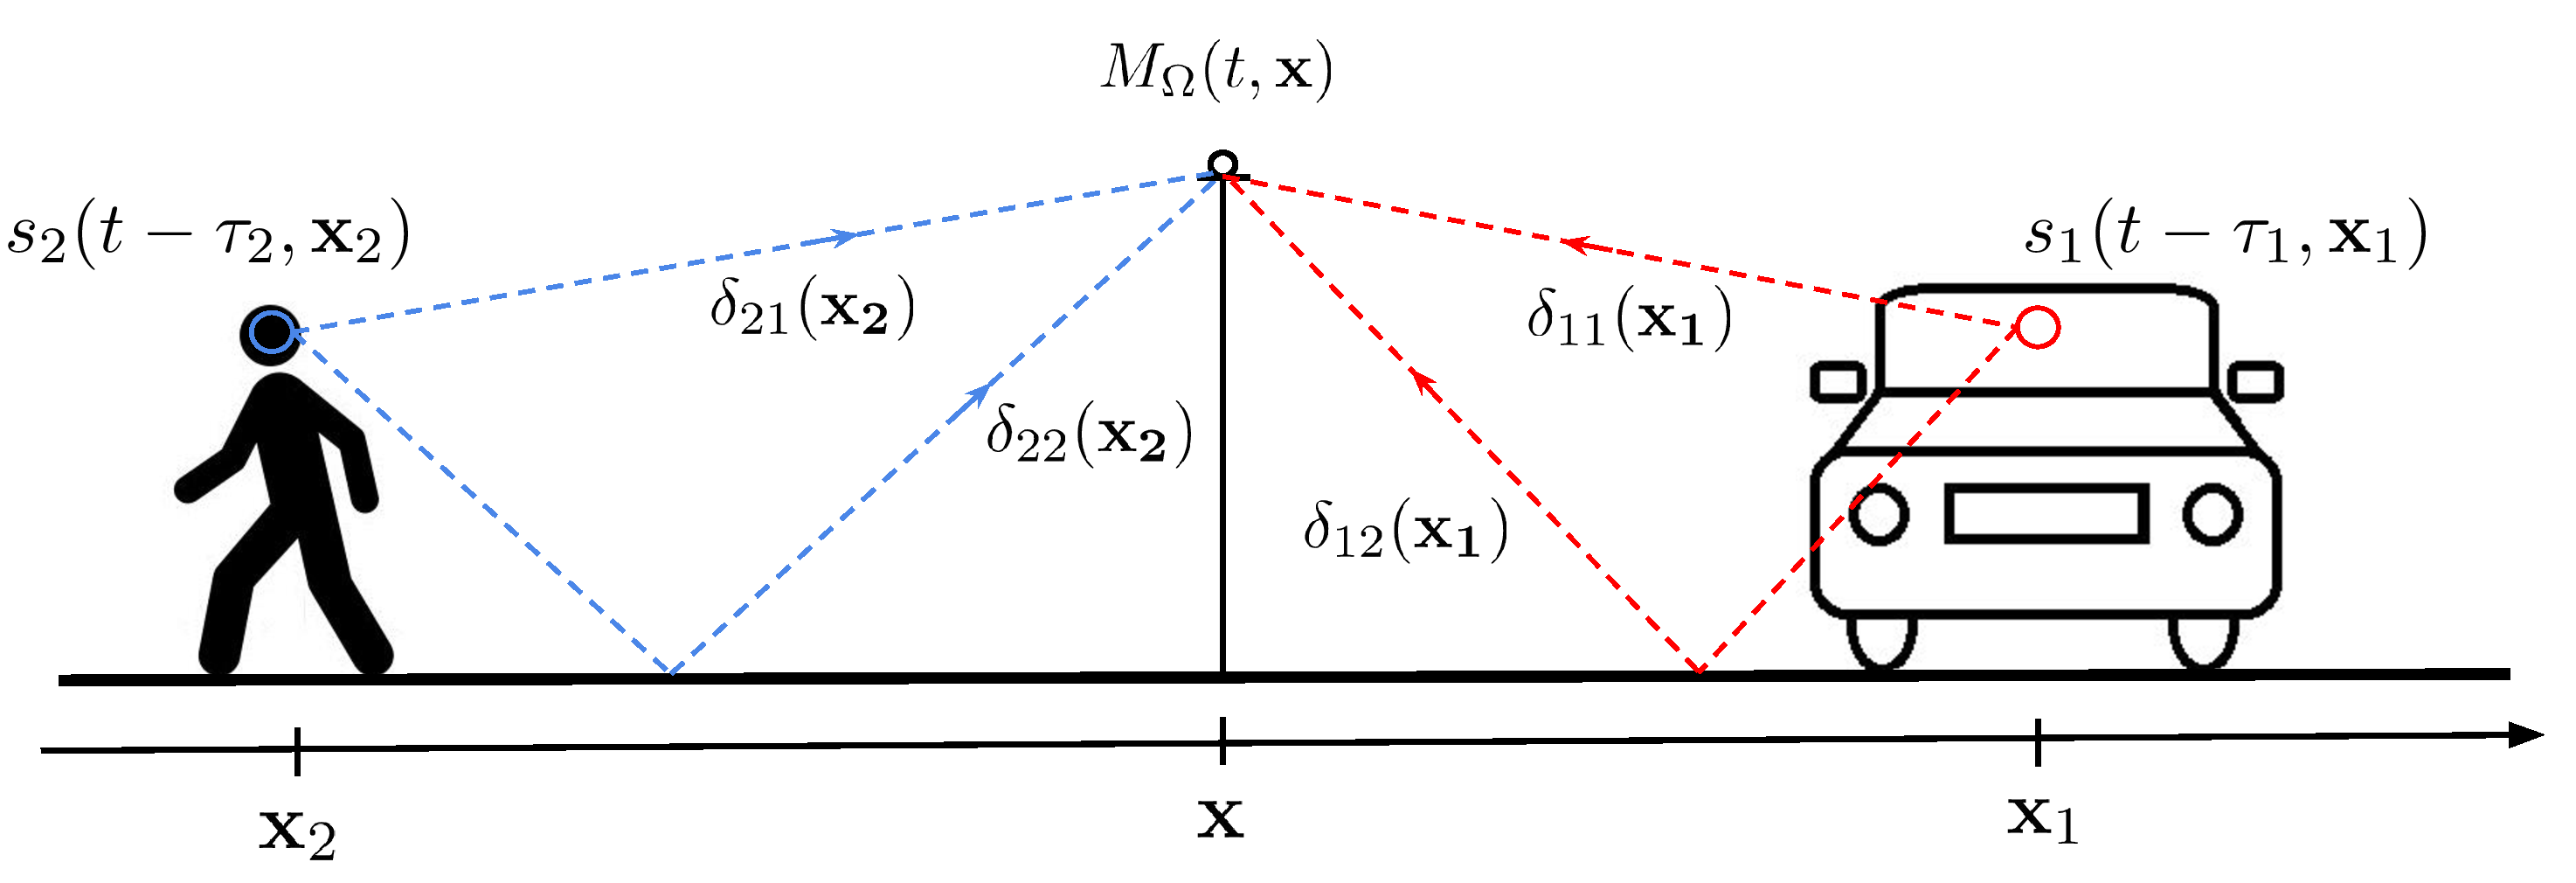
\includegraphics[width=.9\linewidth]{./figures/autres/schema_ville_propa.pdf}
\caption{Schéma du problème considéré en ESU pour un signal capté par un microphone au point $\mathbf{x}$. Deux sources sonores émise à l'instant $t-\tau_{j}$ à la position $x_j$ sont présentes : une voiture, $s_{1}$ (résumée en une source ponctuelle symbolisée par un cercle rouge), et un piéton, $s_2$, (résumée en une source ponctuelle symbolisée par un cercle bleu). Chaque source se propage jusqu'au récepteur selon 2 chemins de propagation (champ direct $\delta_{ij1}$ et champ réfléchi $\delta_{ij2}$).}
\label{fig:schema_ville}
\end{figure}

Les sources $s_j(t)$ expriment les différentes sources sonores présentes en ville comme le trafic aérien ou ferroviaire mais aussi les voix, les bruits de pas, celui d'une valise à roulettes, les sifflements d'oiseaux, les aboiement de chiens \dots{} La source sonore principale en ville est celle du trafic routier qui est considéré comme la somme des contributions des $M$ véhicules présents en ville et dont la somme globale s'exprime :

\begin{subequations}
\begin{align}
S_{tr}(t) &= \sum_{j = 1}^M S_{v_j}(t),\\
 & = \sum_{j = 1}^M s_{v_j}(t-\tau_j) \ast \delta_{j}(t)
\end{align}
\end{subequations}

où $s_{v_j}(t)$ correspond à l'émission sonore du véhicule $j$. L'émission sonore global d'une voiture a plusieurs origines : bruit du moteur thermique, aérodynamique et de roulement. Ici, puisque les citadins ne réalisent pas cette séparation mais considèrent l'ensemble de ces sources comme un tout, on résume la source \textit{voiture} $s_{v_j}(t)$ comme l'ensemble de ses bruits. Précisons que le son émis par le klaxon du véhicule n'est pas considéré dans la source \textit{voiture} car il appartient à la catégorie des avertisseurs sonores.
L'ESU peut ainsi s'exprimer comme  

\begin{equation}
M_i(t) = S_{tr}(t)+\sum_{j = 1}^{N-M}S_j(t),
\end{equation}
\\

qui est un ensemble de sources variées, ayant une allure temporelle, fréquentielle ainsi qu'un niveau sonore propre, et qui sont émises dans un environnement où des phénomènes de propagation complexes ont lieux. Les questions soulevées sont alors : 
 
\begin{itemize}
\item \textbf{Comment caractériser les ESU ? Quels sont les moyens disponibles pour cela ?}
\item \textbf{Comment estimer la présence et le niveau sonore du trafic routier ? Peut-on déterminer la contribution des autres sources sonores ?}\\
\end{itemize}

Avant de répondre à ces questions, il nécessaire, dans un premier temps, d'en présenter les motivations.

\section{De l'intérêt d'étudier les environnements sonores urbains}

Au sein de l'Union Européenne, 70 $\%$ de la population, soit quasiment 340 millions d'habitants, vivent dans des zones urbaines \cite{europ-commission_data_2017}. 486 villes concentrent, chacune, plus de 100 000 habitants. En France, selon l'INSEE, c'est même plus de 84 $\%$ de la population qui vivent dans une zone urbaine, soit plus de 55 millions d'habitants. Cette concentration soulève de grandes questions autour de l'organisation de l'espace urbain afin d'offrir une qualité de vie acceptable aux citadins. En effet, avec de telles densités (environ 3000 habitants/km$^2$ et jusqu'à plus de 21 000  habitants/km$^2$ pour la ville de Paris, la plus dense de l'Union Européenne (UE)), plusieurs formes de pollutions viennent dégrader l'environnement urbain. Des sources de désagrément perçues par le citadin, le bruit est le phénomène qui provoque le plus de gène après la pollution de l'air. Ce bruit est le fruit des activités humaines, provenant essentiellement du transport qu'il soit routier, ferroviaire ou aérien \cite{zannin_characterization_2013}.\\

%\ml{je suis pas trop pour la mise en capitale pour introduire les acronymes}

Selon un rapport de l'Organisation mondiale de la Santé (OMS) \cite{who_burden_2017}, en Europe, près de 200 millions de personnes sont exposées quotidiennement à des niveaux sonores équivalent supérieurs à 55 dB($A$), soit 40$\%$ de la population. Près de 20 $\%$ atteignent même plus de 65 dB($A$) en journée et plus de 30 $\%$ sont touchées par un niveau sonore excédant 55 dB($A$) la nuit. En France, selon un rapport de l'ADEME \cite{europeens2016analyse}, ce sont 52 millions de personnes qui se disent affectées par le bruit et principalement le bruit issu du trafic routier. Plus de 7 millions d'individus sont exposés à des niveaux supérieurs à 65 dB($A$) au quotidien et à plus de 55 dB($A$) la nuit.
Cette exposition quotidienne, à de tels niveaux, n'est pas sans conséquence pour l'être humain. L'impact sur l'organisme humain dû à l'exposition du bruit est observé et étudié depuis de nombreuses années \cite{ising1980health}. Parmi les effets possibles, les plus couramment relevés sont des troubles du sommeil \cite{pirrera2010nocturnal}, de la vigilance et de la concentration, l'augmentation du stress, de la pression artérielle et du rythme cardiaque \cite{babisch2005traffic, babisch2008road}. Selon le rapport de l'OMS, ce sont près de 8 millions de personnes en Europe qui sont affectées par des troubles du sommeil mais aussi 900 000 touchées par de l'hypertension. On estime aussi que 43 000 hospitalisations sont imputables au bruit dues à des pertes de vigilance et de concentration et jusqu'à 10 000 cas de morts prématurées par an. Cet impact sur la santé a également un coût financier pour la société : en France, ce coût est estimé à plus de 11,5 milliard d'euros par an dont une grande partie (89 $\%$) est imputable au bruit du trafic routier \cite{europeens2016analyse}. De plus, si le bruit en ville impacte la vie des citadins, celui-ci se fait également ressentir auprès de la faune sauvage \cite{dutilleux_anthropogenic_2012, francis2009noise} leur causant également du stress ou en compliquant la communication entre les individus et leur reproduction.\\

Le bruit, et une trop grande exposition à celui-ci, a ainsi un impact négatif sur les individus et sur leur environnement. Enjeu de société dont les français ont pleinement conscience \cite{JNA2016etude}, il est nécessaire et utile de caractériser les environnements sonores urbains (ESU) afin d'estimer les sources sonores présentes, leurs niveaux sonores, leurs répartitions et ainsi réduire et limiter leurs impacts sur les populations urbaines.

\section{Utilisation de modèles prédictifs}

L'une des premières pistes pour évaluer les ESU est l'utilisation de modèles prédictifs de bruits de trafic. L'objectif est alors de générer des lois d'émission sonores afin de déterminer les sources $s_j$ et des lois de propagation $\delta_{ij}(t)$. De nombreux modèles d'émission existent afin de prédire les niveaux sonores émis par le trafic routier \cite{quartieri2009review}, ferroviaire \cite{van2000railway} et aérien \cite{zaporozhets1998aircraft}. Étant la source sonore la plus présente et la plus gênante, ce sont les modèles dédiés au trafic routier qui sont ici présentés.

Plusieurs modèles visant à estimer la puissance acoustique, $L_w$, émise par les véhicules et la propagation des ondes sonores dans le milieu urbain ont été développés depuis plus de 30 ans. Plusieurs pays ayant alors leur propre modèle (RLS-90 en Allemagne, CNR en Italie, NMPB-Routes en France, CoRTN au Royaume-Uni, Nord 2000 pour les pays Scandinaves). On se propose tout d'abord de décrire succinctement 3 modèles selon plusieurs paramètres de leur modèle d'émission et de propagation : 

\begin{itemize}
\item Le modèle \bsc{Harmonoise}/Imagine \cite{jonasson2004source}, développé afin d'offrir un premier modèle d'émission harmonisé à l'échelle des pays membres de l'UE. 
\item La NMPB-routes-2008, un modèle français développé à partir des années 90 \cite{setra_prevision_2009-1, setra_prevision_2009-2}. 
\item Le modèle \bsc{Cnossos-Eu}  \cite{CNOSSOS}, le modèle développé le plus récent, là aussi afin d'harmoniser le modèle d'émission sonore et de propagation à l'échelle de l'UE, inspiré par les modèles précédents. 
\end{itemize}

\subsection{Modèle d'émission du trafic routier}\label{part:modele_emission}

Dans ces trois modèles, la puissance émise par une portion de route est lié à la puissance acoustique émise par un véhicule $L_{w,veh}$ et au débit des véhicules $Q$: 

\begin{equation}
L_w = L_{w,veh} + f(Q)
\end{equation}

La puissance acoustique émise par le véhicule est décomposée en deux parties : une composante \og bruit de roulement \fg{}, $L_{w_r}$, et \og bruit de moteur \fg{}, $L_{w_m}$ qui est définie comme 

\begin{equation}
L_{w,veh} = 10\times \log \left(10^{L_{w_r}/10}+10^{L_{w_m}/10}\right)
\end{equation}

Selon le modèle choisi, l'estimation de $L_{w,veh}$ est alors différente. Dans le Tableau \ref{tab:modèle_emission}, les niveaux de puissances $L_{w_r}$ et $L_{w_m}$ et la fonction $f(Q)$ sont exprimés en fonction de la vitesse $v$ du véhicule ainsi que plusieurs paramètres et catégories pris en comptes sont détaillés.

\begin{table}[ht]
\centering
\caption{Paramètre d'estimation de la puissance acoustique selon 3 modèles d'émission sonores}
\label{tab:modèle_emission}
\begin{tabular}{L{2cm}C{4cm}C{4cm}C{4cm}}
 & \bsc{Harmonoise} & NMPB & \bsc{Cnossos-Eu} \\ \toprule
\rowcolor[HTML]{C0C0C0} $L_{w,veh}$ & \begin{tabular}[l]{L{3.5cm}}$L_{w_r} = a_r+b_r\log\left(\frac{v}{70}\right)$ \\ $L_{w_m} = a_m+b_m\left(\frac{v-70}{70}\right)$\end{tabular} &  \begin{tabular}[l]{L{3.5cm}}$L_{w_r} = \alpha_r+\beta_r\log\left(\frac{v}{90} \right)$\\ $L_{w_m} = \alpha_m+\beta_m \log\left(\frac{v}{90} \right)$\end{tabular} & \begin{tabular}[l]{L{3.5cm}}$L_{w_r} = a_r+b_r\log\left(\frac{v}{70}\right)$\\ $L_{w_m} = a_m+b_m\left(\frac{v-70}{70}\right)$\end{tabular} \\ 
$f(Q)$ & $\log\left(\frac{Q}{1000\times v} \right)$ & $\log(Q)$ & $\log\left(\frac{Q}{1000\times v} \right)$ \\
bande de fréquences & 25 Hz - 10 kHz & 100 Hz - 5 kHz & 125 Hz - 4 kHz\\
\rowcolor[HTML]{C0C0C0} description de la source & 2 sources équivalentes ponctuelles & 1 source équivalente ponctuelle & 1 source équivalente ponctuelle \\
nombre de catégorie de véhicule & 5 & 2  & 5 \\
\rowcolor[HTML]{C0C0C0} nombre de revêtement & 1 & 3 & 1 \\
\bottomrule
\end{tabular}
\end{table}

Les valeurs des coefficients dans les modèles \bsc{Harmonoise} et \bsc{Cnossos-Eu}, $a_r$ ,  $b_r$ ,  $a_m$  et $b_m$,   sont données selon les bandes de tiers d'octave et la catégorie du véhicule. Dans la NMPB, $\alpha_r$, $\beta_r$, $\alpha_m$ et $\beta_m$ sont données en fonction de du véhicule, de sa vitesse et du revêtement du sol.
On observe que ces trois modèles, bien que similaire dans leur manière de décomposer la puissance acoustique, présentent plusieurs aspects divergents : nombre de catégorie de véhicules, nombre de revêtement des sols, nombre de bandes de tiers d'octave, calcul d'un niveau en dB pour le modèle \bsc{Harmonoise} et \bsc{Cnossos-Eu} et d'un calcul en dB par mètre pour le modèle NMPB. Ces 3 modèles considèrent des vitesses stables en accélération ou en décélération au travers de corrections qui cependant diffèrent entre les modèles. Si les modèles \bsc{Harmonoise} et \bsc{Cnossos-Eu} sont similaires sur l'estimation des niveaux de puissance $L_{w_r}$ et $L_{w_m}$, le premier considère deux sources ponctuelles pour modéliser un véhicule alors que le second n'en considère qu'une. De plus, dans ces deux modèles si le même nombre de catégories de véhicule est identique, leur classification est différente puisque \bsc{Harmonoise} considère une 5\ieme{} catégorie pour les camions de type tracteur, camion de chantier alors que celle de \bsc{Cnossos-Eu} permet d'inclure les véhicules électriques.

\subsection{Modèle de propagation}\label{part:modele_propa}
Chaque méthode possède également son modèle de propagation acoustique qui simule le rayonnement acoustique de la source. Si le calcul des émissions sonores est très rapide, c'est cet étape qui est la plus longue en raison du volume du domaine à calculer, du nombre de chemin de propagation possible et du nombre de sources sonores à considérer.
Dans le cas du modèle d'\bsc{Harmonoise}, la propagation du son est réalisée en considérant plusieurs approches (résolution de l'équation parabolique, méthode des éléments de frontières ou tir de rayons), afin de s'adapter à différentes configurations, en y considérant des conditions atmosphériques homogènes. L'influence de la route est pris en compte selon son revêtement (température, âge, humidité). Cette approche est reconnue pour être plus \og physique \fg{} mais ausi pour avoir un temps de calcul plus long que les autres modèles (jusqu'à 50 fois plus long) \cite{probst2011comparison}. Pour la NMPB, la méthode de propagation choisie est celle des tirs de rayons où les chemins directs, réfléchis et diffractés sont considérés entre la source et le récepteur. En fonction des conditions atmosphériques relevées (température, vent), les atténuations dans les conditions favorables (à la propagation) et homogènes sont considérées. Les effets de sol (3 types de routes considérés, dont les propriétés varient selon leur ancienneté et la température ambiante de l'air), la divergence géométrique et l'absorption atmosphérique sont aussi prises en compte.
Enfin, les aspects, liés à la propagation du son du modèle NMPB ont été repris dans le modèle \bsc{Cnossos-Eu}. \\
Là encore, les modèles de propagation diffèrent selon les méthodes choisies. Une comparaison plus détaillée entre plusieurs de ces modèles sur de nombreux autres points peuvent être retrouvée dans \cite{steele_critical_2001} et dans \cite{garg_critical_2014}.

\subsection{Réaliser des cartes du bruit de trafic en ville}

À partir de 2002, est instaurée la directive européenne 2002/49/CE \textit{relative à l'évaluation et à la gestion du bruit dans l'environnement} \cite{directive} dont le but est de mieux connaitre la répartition des niveaux sonores générés par le trafic routier, ferroviaire et aérien ainsi que par les Installations Classées pour la Protection de l'Environnement (ICPE) dans les agglomérations de plus de 100 000 habitants. Cette directive prévoit :

\begin{itemize}
	\item d'évaluer l'exposition au bruit des populations basée sur des méthodes communes aux pays européens,
	\item d'informer les populations sur leur niveau sonore d'exposition et sur les effets du bruit sur la santé,
	\item de connaitre et de délimiter les zones bruyantes et les zones calmes.\\
\end{itemize}

Cette directive se traduit notamment par la production de cartes de bruits stratégiques, pour chacune des 4 sources sonores ciblées, afin de déterminer les endroits où les niveaux sonores sont élevés. Un résumé des étapes permettant la réalisation des cartes de bruit du trafic routier est présenté en Figure \ref{fig:cartographie}.\\

% Ces cartes aident ainsi à la mise en place d'aménagements qui permettront de les réduire (construction d'un mur anti-bruit, réduction de la vitesse, mise en place d'un revêtement sol particulier \dots). L'intérêt des modèles prédictifs est alors de pouvoir prédire l'impact de ces aménagements sur l'évolution des niveaux sonores.

\begin{figure}[h]
\centering
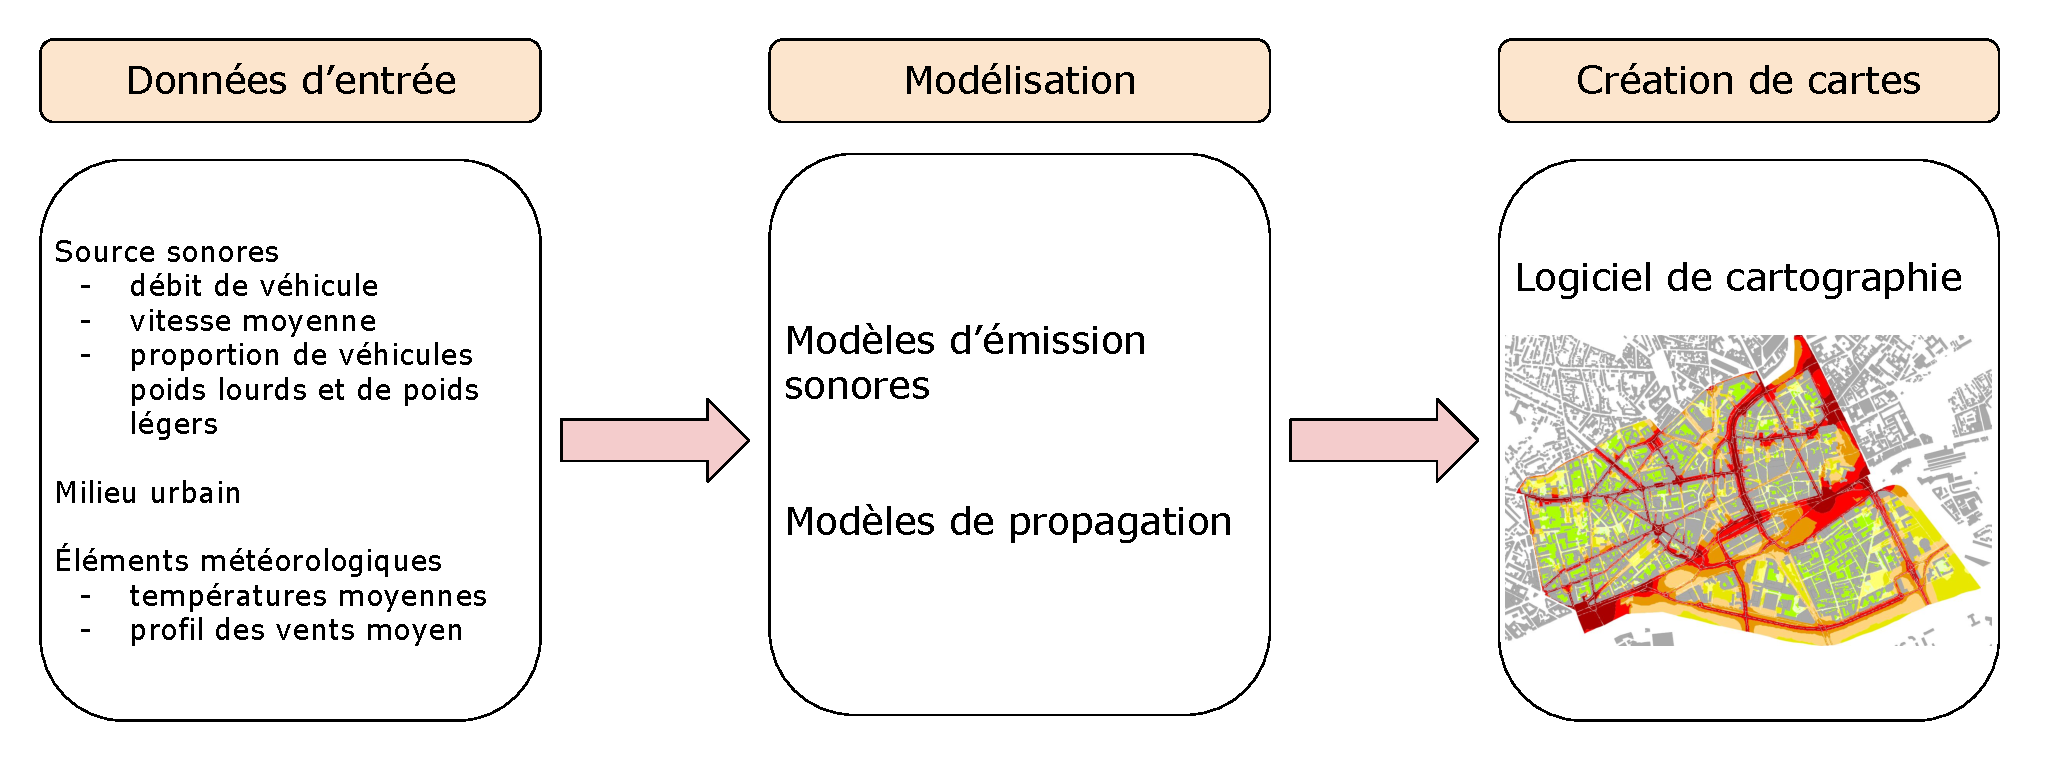
\includegraphics[width=.85\linewidth]{./figures/cartographie/cartographie.pdf}
\caption{Résumé des étapes menant aux cartes de bruit de trafic routier.}
\label{fig:cartographie}
\end{figure}

Dans un premier temps, plusieurs indicateurs en données d'entrée des modèles sont relevés \textit{in situ} :  

\begin{itemize}
\item vitesses moyennes des véhicules sur les portions de routes principales,
\item débits de véhicules (nombre de véhicules par tranche horaire),
\item composition du trafic (nombre de véhicules légers et de poids lourds).
\item architecture et topographie de la ville (revêtement au sol), 
\item conditions météorologiques (températures, vent).\\
\end{itemize}

\begin{figure}[t]
\centering
\subfigure[\label{fig:lden}]{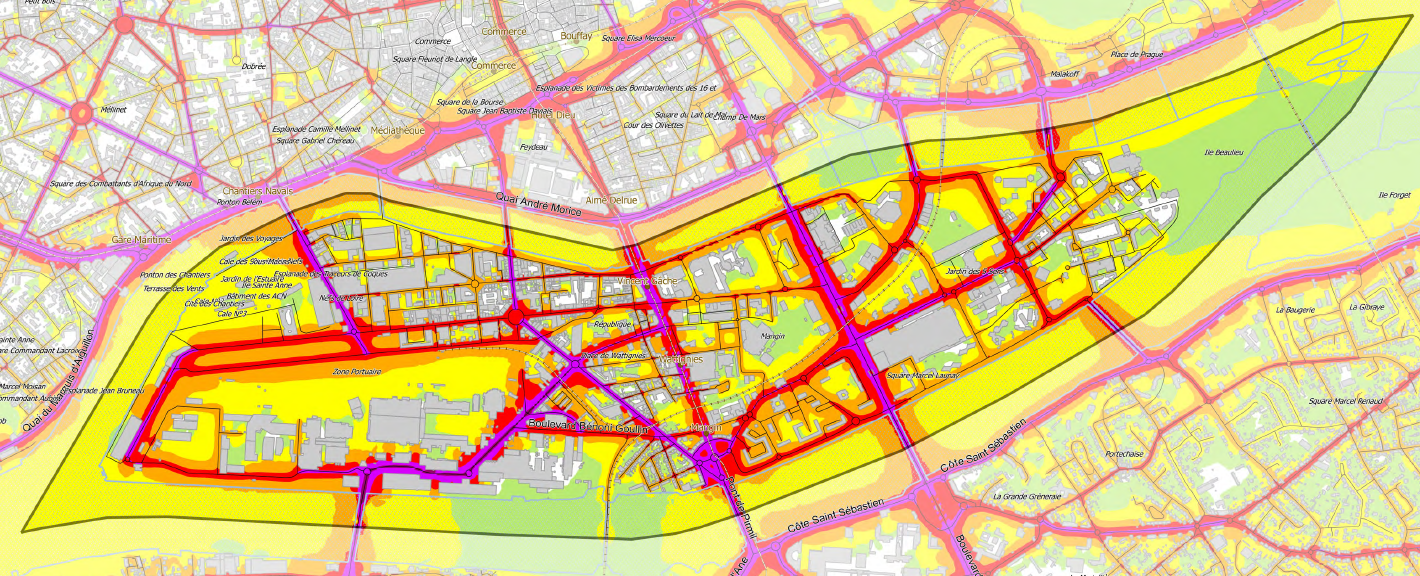
\includegraphics[width=0.85\linewidth]{./figures/cartographie/Lden_ile_Nantes.PNG}}
\subfigure[\label{fig:ln}]{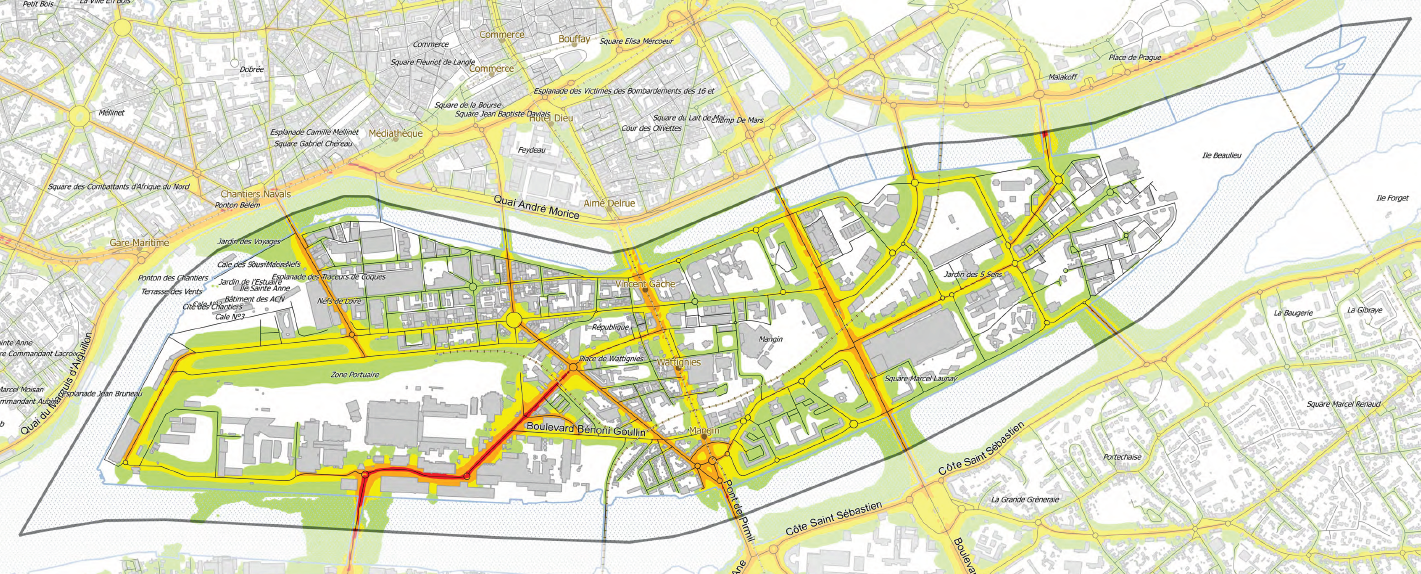
\includegraphics [width=0.7\linewidth]{./figures/cartographie/Ln_ile_Nantes.PNG}}
\caption{$L_{DEN}$ \subref{fig:lden} et $L_N$ \subref{fig:ln} de l'île de Nantes pour le trafic routier \cite{nantes_carte}.}
\label{fig:carto_nantes}
\end{figure}

Puis à partir d'un modèle d'émission sonore et de ces données d'entrée, il est possible d'établir la puissance émise par chaque véhicule, $s_{v}(f)$.
Enfin, l'influence de l'environnement $\delta(t)$ sur la répartition des niveaux sonores dans la ville est calculé à l'aide d'un logiciel numérique (Mithra, Immi, CadnAa \dots). Les logiciels accompagnés d'un Système d'Information Géographique (SIG) sont ceux qui offrent actuellement le plus de possibilités. Un SIG est un outil informatique conçu pour stocker, analyser et manipuler plusieurs type de données spatiales et géographiques comme l'architecture des villes ou le nombre d'habitants présents. 
Son utilisation permet alors de connaitre plus facilement le nombre de citadins exposés à des forts niveaux sonores. 
Par exemple, le logiciel OrbisGIS\footnote{\url{http://orbisgis.org/}}, destiné à représenter de données spatiales, permet la réalisation de cartes de bruit à l'aide de l'ajout d'un plugin, \textit{NoiseModelling}, développé par \cite{fortin}. \\

Les cartes de bruits produites résument les niveaux sonores équivalent pondérés $A$ sur 24h ($L_{DEN}$ pour \textit{Day-Evening-Night} (\textit{Jour-Soir-Nuit} en français)) et durant la nuit ($L_N$) :

\begin{equation}
L_{DEN} = 10\times\log \left(\frac{1}{24} \left(12\times10^{\frac{L_D}{10}}+4\times10^{\frac{L_E+5}{10}}+8\times10^{\frac{L_N+10}{10}} \right)\right)
\end{equation}

avec $L_D$, $L_E$ et $L_N$, les niveaux sonores équivalent pondéré $A$ pour les périodes respectives 6h-18h, 18h-22h, 22h-6h (horaires pouvant être changées suivant le rythme de vie des habitants de la zone considérée),

\begin{subequations}
\begin{align}
L_D &= 10\times\log\left(\frac{1}{T} \sum_{t = 1}^{T}10^{\frac{L_{D_t}}{10}}\right),\\
L_E &= 10\times\log\left(\frac{1}{T} \sum_{t = 1}^{T}10^{\frac{L_{E_t}}{10}}\right),\\
L_N &= 10\times\log\left(\frac{1}{T} \sum_{t = 1}^{T}10^{\frac{L_{N_t}}{10}}\right)
\end{align}
\end{subequations}

avec $L_{X_t}$, le niveau sonore dans la tranche horaire $t$. Les niveaux $L_E$ et $L_N$ sont majorés respectivement de 5 dB($A$) et de 10 dB($A$) afin de pénaliser les plages horaires où la gêne occasionnée par le trafic est plus importante. La Figure \ref{fig:carto_nantes} résume, par exemple, le $L_{DEN}$ et le $L_N$ pour le bruit du trafic routier dans un quartier de la ville de Nantes.
La réalisation de ces cartes permet alors d'estimer le nombre  de personnes touchées par ces niveaux sonores élevés et facilite ainsi la mise en oeuvre de travaux d'aménagement (construction de mur anti-bruit, changement de revêtement, diminution des vitesses \dots) si les niveaux sonores mesurés sont trop élevés selon la réglementation en vigueur. L'utilisation de modèles prédictifs présente alors l'intérêt de pouvoir simuler l'effet de ces dispositifs sur les niveaux sonores émis et d'en mesurer l'impact \cite{murphy2011scenario,guedes2011influence}. Les cartes produites doivent ensuite être mises à jours tous les 5 ans.


\subsection{Vers la modélisation d'autres sources sonores ?}

Le trafic routier, aérien et ferroviaire et les ICPE sont actuellement les seules sources sonores à faire l'objet de cartes de bruit. Mais il est tout à fait possible d'ouvrir ces outils à d'autres sources sonores. 
En effet, les cartes de bruits, si elles permettent de mieux identifier la présence de bruits en ville, ne permettent pas de représenter au mieux la perception des citadins de l'ESU \cite{brown2012review}. Plusieurs sources sonores aux travers d'études perceptives ont montré leur influence dans la perception de l'ESU comme la voix, le chant d'oiseaux, le bruit des fontaines \cite{lavandier2006contribution,hong2013designing}. 
Il peut donc être intéressant et utile de savoir estimer leur présence dans les villes afin de permettre une représentation des ESU non plus juste à partir d'indicateurs physiques de sources sonores connotées négativement (comme le trafic routier) mais également des sources plus appréciées.  
Certaines sources sonores ont déjà fait l'objet de modélisation (dans le cadre d'autres études ou applications) comme les oiseaux \cite{nemeth2013bird}, les voix \cite{hayne2011prediction} ou les fontaines \cite{watts2009measurement}, mais ne sont, pour l'instant pas assez étudiées pour offrir des modèles validés. 
Une des difficultés est la localisation de certaines de ces sources dans l'espace urbain. Si les sources sonores fixes comme les fontaines ou les cloches d'une église sont faciles à localiser, d'autres, comme la foule et les oiseaux, sont plus difficiles à déterminer car plus mobiles et parcimonieuses. Dans \cite{aumond2018probabilistic}, c'est par une approche statistique que la position des sources est déterminée : les piétons sont ainsi plus susceptible de se trouver sur des places ou le long des trottoirs, dans les parcs ou auprès des arbres pour les oiseaux. Il deviendrait alors envisageable de générer des cartes dites multi-sources d'une ville où une représentation des niveaux sonores émis par chaque source pourrait être générée et ainsi s'orienter vers des cartes de bruits perceptives.

%De plus, à partir des études perceptives réalisées, il deviendrait possible de lier les niveaux physiques prédit à des indicateurs perceptifs et ainsi générer des cartes de bruits perceptives qui serait lié à la perception du citadin de son environnement. Dans \cite{aumond2017modeling}, l'évaluation perceptive de citadins d'ESU est corrélé à des indicateurs physiques deux modèles d'agrément sonore sont proposés issus d'enregistrements sonores et des évaluations perceptives de citadins. L'un se base sur des grandeurs physiques tels que le niveau sonore fractile $L_{50}$ dans la bande de tiers d'octave de 1 kHz ainsi que la variation normalisée en temps et en fréquence des bandes de 500 Hz et de 4 kHz 
%Dans \cite{aumond2017modeling}, cet agrément sonore, déterminée par une marche sonore (ou \textit{soundwalk}) auprès de citadins dans la ville de Paris, y est corrélée au niveau sonore globale de la scène sonore et au temps de présence du trafic, de la voix et des oiseaux. \\


\subsection{Limitations des modèles prédictifs}

L'utilisation de modèles d'émissions sonores présente donc plusieurs intérêts : prédiction des niveaux sonores dans une situation donnée, création de cartes de bruit de trafic et possibilité de tester différents scénarios d'aménagements. Leur utilisation s'est répandue et démocratisée en raison de l'introduction de la directive européenne. Les premières études réalisées suivant les recommandations de la directive ont permis de soulever plusieurs limites à cette méthode comme celles lié au choix du modèle parmi ceux existants, aux incertitudes liées aux estimations des données d'entrées.

\subsubsection{Limites liées à la modélisation de la source et de la propagation}

Ces modèles sont basés sur des mesures et des études physiques du trafic. Comme tout modèle simulant la réponse d'un système physique, il n'est pas possible d'en générer un universel qui puisse s'adapter à l'ensemble des cas et scénarios possibles. Des simplifications sont ainsi réalisées, par exemple en classifiant les routes et le parc automobile en un nombre réduit de catégories ou bien en considérant (ou non), en plus des conditions atmosphériques homogènes, des conditions favorables à la propagation. Ce sont d'autant plus de simplifications qui, certes, facilite l'implémentation et l'utilisation des modèles mais qui sont aussi vecteurs d'incertitudes. De plus, ces catégorisations prennent le risque de mal prendre en compte certain cas limites qui ne correspondent pas spécifiquement à ceux définis.

Un second aspect, évoqué dans les parties \ref{part:modele_emission} et \ref{part:modele_propa} est celui de l'existence de plusieurs modèles d'émission et de propagation au sein de plusieurs pays européens. Avant même la mise en place de la directive, \cite{steele_critical_2001} en avait comparé plusieurs selon différents aspects (données d'entrée, type de cartographie, méthode de propagation des différents logiciels). 
Parmi ces différents outils, l'auteur met en avant le problème, soulevé également par \cite{king_implementation_2011}, de la diversité des méthodes de calculs qui peuvent être employées : quelle méthode, parmi celles existantes, doit-être utilisée ? 
Dans un premier temps, ce choix a été laissé libre par la directive européenne. Les premières cartes de bruits ont donc été établies sur des modèles différents : par exemple pour la même année, dans \cite{kliuvcininkas2006noise}, le modèle RLS-90 est employé pour calculer la carte de bruit dans le centre-ville de Kaunas, en Lituanie,  alors que dans \cite{murphy_environmental_2006}, la carte de bruit de trafic dans la ville de Dublin, en Irlande, est construite sur la base du modèle \bsc{Harmonoise}. 
Une comparaison exhaustive de 8 modèles (FHWA, CoRTN, RLS-90, ASJ, \bsc{Harmonoise}/Imagine, Son Road, Nord 2000 et NMPB-Routes-2008) a également été réalisée par Garg et Maji \cite{garg_critical_2014} selon un plus grand nombre de critères (modélisation des sources sonores, vitesse des véhicules (constantes, accélération/décélération, intersection\dots), modèle de propagation, modélisation des effets de sol, effets météorologiques \dots). À travers leur comparaison, les auteurs relèvent ainsi les nombreuses différences entre les modèles notamment auprès des modèles de propagations du son. Les auteurs de l'étude précise tout de même qu'il est difficile de déterminer un \og meilleur \fg{} modèle par rapport aux autres, chacun ayant une approche différente. 
Afin de résoudre ces problèmes, la méthode \bsc{Cnossos-Eu} \cite{CNOSSOS,kephalopoulos} a ainsi été développée, basée sur les méthodes déjà existantes en vue d'harmoniser la construction des cartes de bruit des villes à l'échelle européenne permettant plus facilement leur comparaison. 

Si l'harmonisation des méthodes est bénéfique, la confrontation des modèles face à des mesures faites en villes reste toutefois à être réalisée. L'ensemble de ces modèles d'émission et de propagation a été développé et validé à partir de mesures faites dans des conditions optimales. Toutefois, la comparaison entre les niveaux sonores calculés et mesurés reste délicate. Premièrement, les mesures présentent l'inconvénient d'être soumises à d'autres sources sonores qui ne sont pas liées au trafic et qui viennent donc détériorer les mesures. De plus, il faut s'assurer, lors des mesures, que les données d'entrée fournies aux modèles correspondent bien aux conditions expérimentales ce qui n'est pas facile.

Enfin, ces modèles dépendent des données d'entrée relevées \textit{in situ} s'exprimant sous la forme de moyennes et qui induisent donc des écarts-types qui se propagent dans les étapes suivantes du calcul. La propagation de ces écarts-types a été étudiée dans \cite{probst2005uncertainties}, l'auteur y concède qu'estimer une incertitude $\sigma$ à un niveau sonore à un point donné est un processus long et difficile.

\subsubsection{Limites liées à la simulation et à la représentation}

Dans le cas de la cartographie de bruit, les modèles de sources et de propagation sont implémentés dans des logiciels pour déterminer, sur l'ensemble d'une ville ou d'un quartier, les niveaux sonores liés au trafic. Cette tâche peut être très lourde en coût et en temps de calculs (de quelques heures à plusieurs jours). Pour cela, l'utilisateur a la possi

Tout d'abord, l'environnement urbain est simplifié en le discrétisant, le plus souvent par un maillage régulier de 10 mètres par 10 mètres. À l'échelle d'une ville, c'est ainsi plusieurs millions de points qui peuvent être définis. Chaque point source est alors rattaché à un point du maillage et le calcul consiste ensuite à estimer la propagation acoustique entre les sources et les points de ce maillage, selon les différents chemins de propagation possibles, pour chaque bande de fréquence. Le nombre de chemin considéré est également défini par l'utilisateur, ce qui selon la valeur choisie, influe sur la quantité d'énergie final présente en un point $i$ mais également sur le temps de calcul.
 
L'étape de discrétisation du milieu, si elle simplifie la forme de l'environnement urbain, présente l'inconvénient de ne pas prendre en compte les multiples variations géométriques des façades ou bien l'ensemble des petits mobiliers urbains qui ont un rôle dans la diffusion du son. 
De plus, en raison de la discrétisation du milieu, des méthodes d'interpolation (méthode linéaire, de krigeage) sont utilisées pour calculer les niveaux sonores entre ces points, ce qui est également source d'approximation qui peuvent mener à de mauvaises interprétations \cite{van_leeuwen_noise_2015}.

Enfin, une fois la carte générée, on peut noter que seulement 2 niveaux sonores par source de trafic sont obtenus, $L_{DEN}$ et $L_N$, et mis à jour tous les 5 ans seulement. C'est donc une information statique et restreinte que la directive européenne impose. Cependant, le trafic routier, ferroviaire et aérien varient aussi bien à l'échelle de l'année, d'une journée ou même d'une heure \cite{lv2015traffic}. S'il parait envisageable de calculer des cartes de bruit pour, par exemple, chaque heure de la journée, cela reste une opération très longue et couteuse à réaliser.
L'utilisation de modèles dynamiques de trafic, couplés aux modèles d'émissions sonore  \cite{can2010traffic}, n'est actuellement pas destiné à la cartographie des ESU mais est une piste envisageable pour lier les interactions entre les véhicules et leur cinématique à l'échelle d'une rue ou d'un quartier.

En conclusion, l'utilisation de modèles prédictifs est une approche utile pour réaliser une première estimation de la répartition du bruit de trafic en ville. Si elle présente des avantages (estimation d'un niveau physique à l'échelle de la ville, possibilité de tester des scénarios d'aménagement), elle présente plusieurs limites : 

\begin{itemize}
\item le nombres de sources est, pour l'instant, trop restreint et ne permet pas de considérer l'ensemble des ESU et la perception qu'en ont les citadins,
\item l'utilisation d'un modèle d'émission et de propagation et la calcul numérique entraine de nombreuses incertitudes qui sont difficiles à estimer, 
\item l'accès à l'évolution temporelle des sources sonores n'est pas possible.
\end{itemize}

Afin de considérer l'ensemble des sources et des évènements sonores présents en ville et de compléter les estimations générées par les modèles prédictifs, une autre approche est envisagée, basée sur la réalisation de mesures et d'enregistrements sonores réalisés directement dans la ville.

\section{Utilisation de mesures acoustiques}

À la différence des modèles prédictifs qui déterminent l'émission sonore des sources $s_j(t)$ et leur propagation $\delta_{ij}(t)$ pour en déterminer le niveau sonore en un point $i$, la réalisation de mesures donne directement accès à la mixture globale $M_{i}(t)$. Les limites liées à la modélisation des sources, de la propagation du son et de l'ensemble des environnements urbains dans toute leur complexité n'interviennent alors plus dans les mesures faites \textit{in situ}.

De nombreuses études ont déjà été menées en ville en faisant intervenir des mesures pour des durées plus ou moins longues (de quelques jours \cite{romeu2011street} à plusieurs années \cite{gaja2003sampling}) avec des microphones de mesures de hautes qualités. Dans une première étude \cite{zannin2002environmental} a réalisé une série de mesures sur près de 1000 positions dans la ville de Curitiba, au Brésil, pour étudier l'ESU dans sa globalité afin d'évaluer l'exposition aux bruits dans les différents quartier de la ville, puis a réduit la surface d'étude dans \cite{zannin_characterization_2013} où 58 points de mesures sont déployés dans le campus universitaire de la ville. 
Dans \cite{Mioduszewski}, 40 microphones sont placés isolément à travers la ville de Gdansk en Pologne pour une durée d'un an afin d'y mesurer le niveau sonore du trafic et de valider la cartographie de bruit. 

Si ces mesures ont eu une durée de vie limitée dans le temps, la pérennisation de l'installation de capteurs en ville est de plus en plus envisagée à l'heure de l'émergence de l'\textit{IoT} (\textit{Internet of Things} ou l'internet des objets en anglais) \cite{zanella2014internet} et de la ville intelligente (\textit{Smart City} en anglais) \cite{chourabi2012understanding}. De nombreuses villes s'équipent actuellement en réseaux de différents types de capteurs disséminés dans le milieu urbain afin d'en contrôler, en temps réel, de nombreux aspects : distribution d'énergie, gestion des transports, de l'eau ou des déchets. L'objectif étant alors d'optimiser le fonctionnement de la ville afin d'améliorer la qualité de vie des citadins. L'arrivée sur le marché de capteurs acoustiques à bas coût (moins de 10 € pour un capteur microphone MEMS) \cite{van2010use} rend alors possible le déploiement de capteurs acoustiques dans ces réseaux. La mise en place de tels réseaux en villes donne lieux à plusieurs projets où différentes approches sont étudiées : nombre de capteurs installé, surface couverte par ce réseau, mesures fixes ou mobiles \dots

\subsection{Déploiement de réseaux de capteurs fixes}

Ces réseaux sont constitués d'un ensemble de capteurs fixes alimentés et connectés à un réseau de télécommunication. Leurs mesures sont alors stockées par des serveurs pour ensuite être post-traitées. L'intérêt principal d'un tel réseau est la possibilité d'avoir accès à des variations à long-terme des niveaux sonores à l'emplacement des microphones. Un schéma d'un tel réseaux est résumé en Figure \ref{fig:reseau_capteur}.

\begin{figure}[t]
\centering
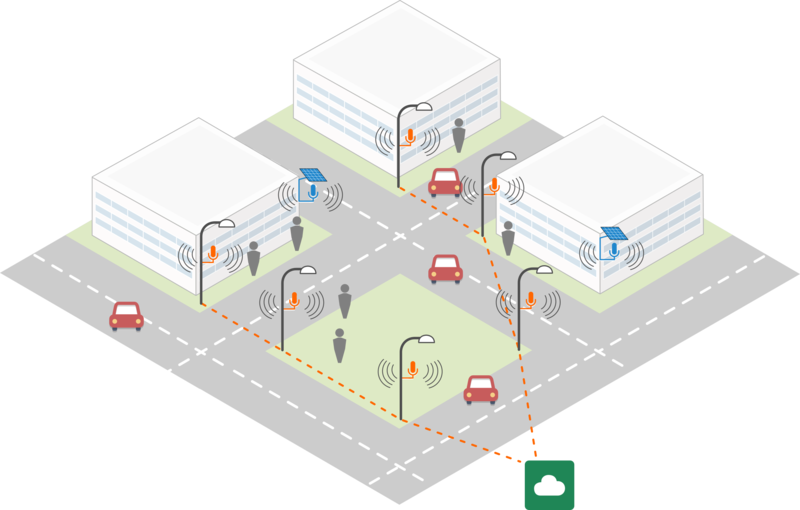
\includegraphics[width=0.8\linewidth]{./figures/cartographie/reseau_mesure.png}
\caption[Schéma d'un réseau de capteurs fixes]{Schéma d'un réseau de capteurs fixes\protect\footnotemark}
\label{fig:reseau_capteur}
\end{figure}

\footnotetext{\url{http://cense.ifsttar.fr/}}

Un premier réseau de capteurs développé depuis plusieurs année est celui de la ville de Paris, géré par BruitParif, à travers le projet RUMEUR \cite{mietlicki2012innovative}, qui existe déjà depuis plusieurs années, où des réseaux de microphones sont déployés afin d'évaluer l'ESU en région parisienne. Le réseau comprend des stations fixes mais intègre aussi des campagnes de mesures plus courtes (de plusieurs heures à plusieurs années) pour voir l'impact acoustique d'un évènement (journée sans voiture) ou d'un aménagement (modifications de voirie). Un site internet\footnote{\url{http://rumeur.bruitparif.fr/}} est mis à disposition pour avoir un aperçu complet des mesures réalisées sur les nombreux emplacements.
En parallèle, plusieurs études se sont intéressées à la prise en compte de mesures pour caractériser le bruit du trafic comme dans \cite{makarewicz_empirical_2011} qui propose une estimation des niveaux sonore $L_{DEN}$ et $L_N$ directement à partir des mesures et dont son incertitude est estimée en fonction de la durée d'acquisition des mesures. Dans \cite{wei_dynamic_2016}, une technique d'assimilation de données est proposée afin de réaliser des cartes de bruit dynamiques basées sur des mesures. Les niveaux de puissances et les effets de propagation de chaque source sont ici modifiés par des termes correctifs obtenus en minimisant l'erreur au carré entre les niveaux prédits et les niveaux mesurés.

\`A l'heure actuelle, plusieurs projets étudient la mise en place de réseaux plus important comme le projet européen DYNAMAP \footnote{\url{http://www.life-dynamap.eu/}} \cite{dynamap_2016}. Ce projet a pour objectif de développer un système de cartographie de bruit dynamique basé sur des réseaux de capteurs à bas coûts installés en ville. Une application de ce projet a déjà été réalisée dans deux villes tests, Milan et Rome \cite{bellucci_life_2017}.
Le principe de leur approche est d'ajuster les cartes de bruits simulées à partir des différences obtenues entre les niveaux sonores mesurés aux stations et les niveaux sonores calculés à ce même point par les modèles prédictifs. Pour limiter le coût d'un tel déploiement, le nombre de microphones est réduit en les installant à des emplacements spécifiques représentatifs des différents scénarios possibles de trafic routier (homogénéité du trafic, type de revêtement) \cite{zambon2017life}.
Le projet SONYC \footnote{\url{https://wp.nyu.edu/sonyc/}} à New-York dédie son réseau de capteurs à la surveillance de la pollution sonore et au développement d'outils de traitement du signal afin de décrire l'ESU par l'étude des sources présentes \cite{mydlarz2017noise}. 
Enfin, le projet CENSE\footnote{\url{http://cense.ifsttar.fr/}} vise à développer un réseau de capteurs dans la ville test de Lorient afin là encore d'améliorer la cartographie du bruit de trafic en agrégeant les données simulées des niveaux sonores du trafic avec les mesures réalisées en ville par ce réseau. L'approche est différente de DYNAMAP, puisqu'ici l'étude se restreint à l'échelle de plusieurs quartiers de la ville afin d'avoir un réseau de capteurs dense. La mise à jour des cartes est faite à l'aide de techniques d'assimilation de données en vue de compléter les cartes de bruits prédites avec les mesures.
Ces méthodes d'assimiliation sont notamment utilisés dans le domaine des sciences géophysiques et consistent à modifier une estimation émises par un modèle prédictif à partir de données mesurées \cite{wu2008comparison}.
Le projet s'intéresse également à la perception des citadins des ESU aux travers de questionnaires qui leur sont envoyés et des mesures réalisées par ce réseau de capteurs.

L'utilisation de ces mesures faites en villes est donc variable (cartographie dynamique du bruit de trafic, études perceptives, détection d'évènements anormaux ou dont le niveau sonore est supérieur à ceux défini par des réglementations). Toutefois, l'installation de tels réseaux de capteurs nécessite de gérer de nombreuses problématiques techniques comme la disposition des microphones, leur maintenance, la transmission et le stockage des mesures, leur alimentation électrique\dots{} Une des première limite technique est la performance individuelle des capteurs. En effet, la réduction de leur coût s'est faite en diminuant leur performance  individuelle (dynamique énergétique et fréquentiel) \cite{mydlarz2015design}. Il est donc nécessaire de caractériser chacun des microphones en vue de connaitre leurs performances et leur limites.
Mais une des points cruciaux est celui de la position des microphones des mesures (quelle hauteur ? quelle position par rapport à des sources sonores qui seraient digne d'intérêts ?) et de la surface couverte par ces mesures. Un réseau distribué selon un maillage dense permettra une bonne représentation de l'espace mais coutera cher à installer et à maintenir alors qu'une faible densité de capteurs sera moins onéreuse mais apportera moins d'information et nécessitera des interpolations entre les mesures, ce qui reste une source d'incertitudes.
Toutefois, la réalisation de mesures acoustique en ville n'est pas nécessairement obligée d'être réalisée via des réseaux de capteurs fixes. D'autres pistes sont également explorées.

\subsection{Mesures mobiles}

En parallèle aux réseaux fixes, la mesure mobile est une voie envisagée. Elle consiste à réaliser des mesures acoustiques en plaçant le microphone sur un support mobile (piéton, cycliste, voiture, bus). 

Dans le cadre des études des ESU et du bruit de trafic, l'avantage de cette méthode par rapports aux capteurs fixes est sa capacité à pouvoir couvrir plus facilement une plus grande surface urbaine à moindre coût. Les mesures mobiles sous-entendent deux manières d'être réalisées : soit le microphone réalise sa mesure sur un support mobile qui se déplace en même temps \cite{alsina-pages_design_2016}. Dans ce cas, un traitement du signal doit être effectué pour prendre en compte le bruit émis par ce support, soit le support permet de déplacer le microphone pour faire ensuite des mesures fixes \cite{manvell2004sadmam} ce qui simplifie la tâche mais qui nécessite plus de temps pour couvrir une surface similaire par rapport aux mesures faites sur un support mobile.
L'inconvénient de ces méthodes est qu'elle ne permettent pas la réalisation de mesures à long terme et donc de ne pas pouvoir estimer l'évolution temporelle des niveaux sonores en un point donné au cours du temps.
En conséquence, plusieurs travaux se sont intéressés à l'agrégation des mesures mobiles à des mesures réalisées par des stations fixes.
\cite{morillas2014uncertainty} s'intéresse aux incertitudes sur l'estimation des niveaux sonores estimés suivant le nombre de points ou de jours de mesures. Dans \cite{can_measurement_2014}, la prise en compte de mesures mobiles pour compléter des stations fixes est comparé à des méthodes d'interpolation (méthode de Kriging , pondération inverse de la distance). Il en résulte que l'apport des mesures mobiles diminue l'erreur produite par rapport aux méthodes d'interpolation en cela qu'elles permettent d'apporter plus d'informations quant aux variations spatiales du niveau sonore (rues calmes peu fréquentées, rues très passantes, aux abords d'intersections\dots) ce que ne permet pas une méthode d'interpolation numérique \cite{aumond2018kriging}.

La réalisation de mesures mobiles est notamment très courante pour des études perceptives de l'ESU par des citadins lors de \textit{soundwalks} (\textit{marche sonore} en français). Cette méthode consiste à réaliser un parcours en ville et à soumettre, à un panel d'auditeur, un questionnaire sur les sons qui les entourent. L'enregistrement de l'ESU durant cette marche permet alors de corréler leurs réponses et leur perception avec des indicateurs (niveau sonore en dB($A$), présence de certaines sources sonores \dots{}) extraits de ces enregistrements \cite{brocolini_measurements_2013, hong2013designing}). Dans \cite{aumond2017modeling}, l'évaluation perceptive d'ESU par des citadins est corrélée à des indicateurs physiques tels que le niveau sonore fractile $L_{50}$ dans la bande de tiers d'octave de 1 kHz ainsi que la variation normalisée en temps et en fréquence des bandes de 500 Hz et de 4 kHz.
Enfin, les mesures mobiles peuvent servir à des études plus ponctuelles par exemple en vue de classer les ESU selon différents indicateurs physiques comme dans \cite{rychtarikova2013soundscape}, où 370 enregistrements 15-20 minutes réalisés dans 4 villes de Belgique ont été réalisés lors de \textit{marche sonore}, et dans \cite{can_describing_2015}, où des enregistrements mobiles ont été réalisés dans la ville de Marseille.

\begin{figure}[t]
\begin{center}
    \begin{minipage}[t]{0.3\textwidth}
        \centering
        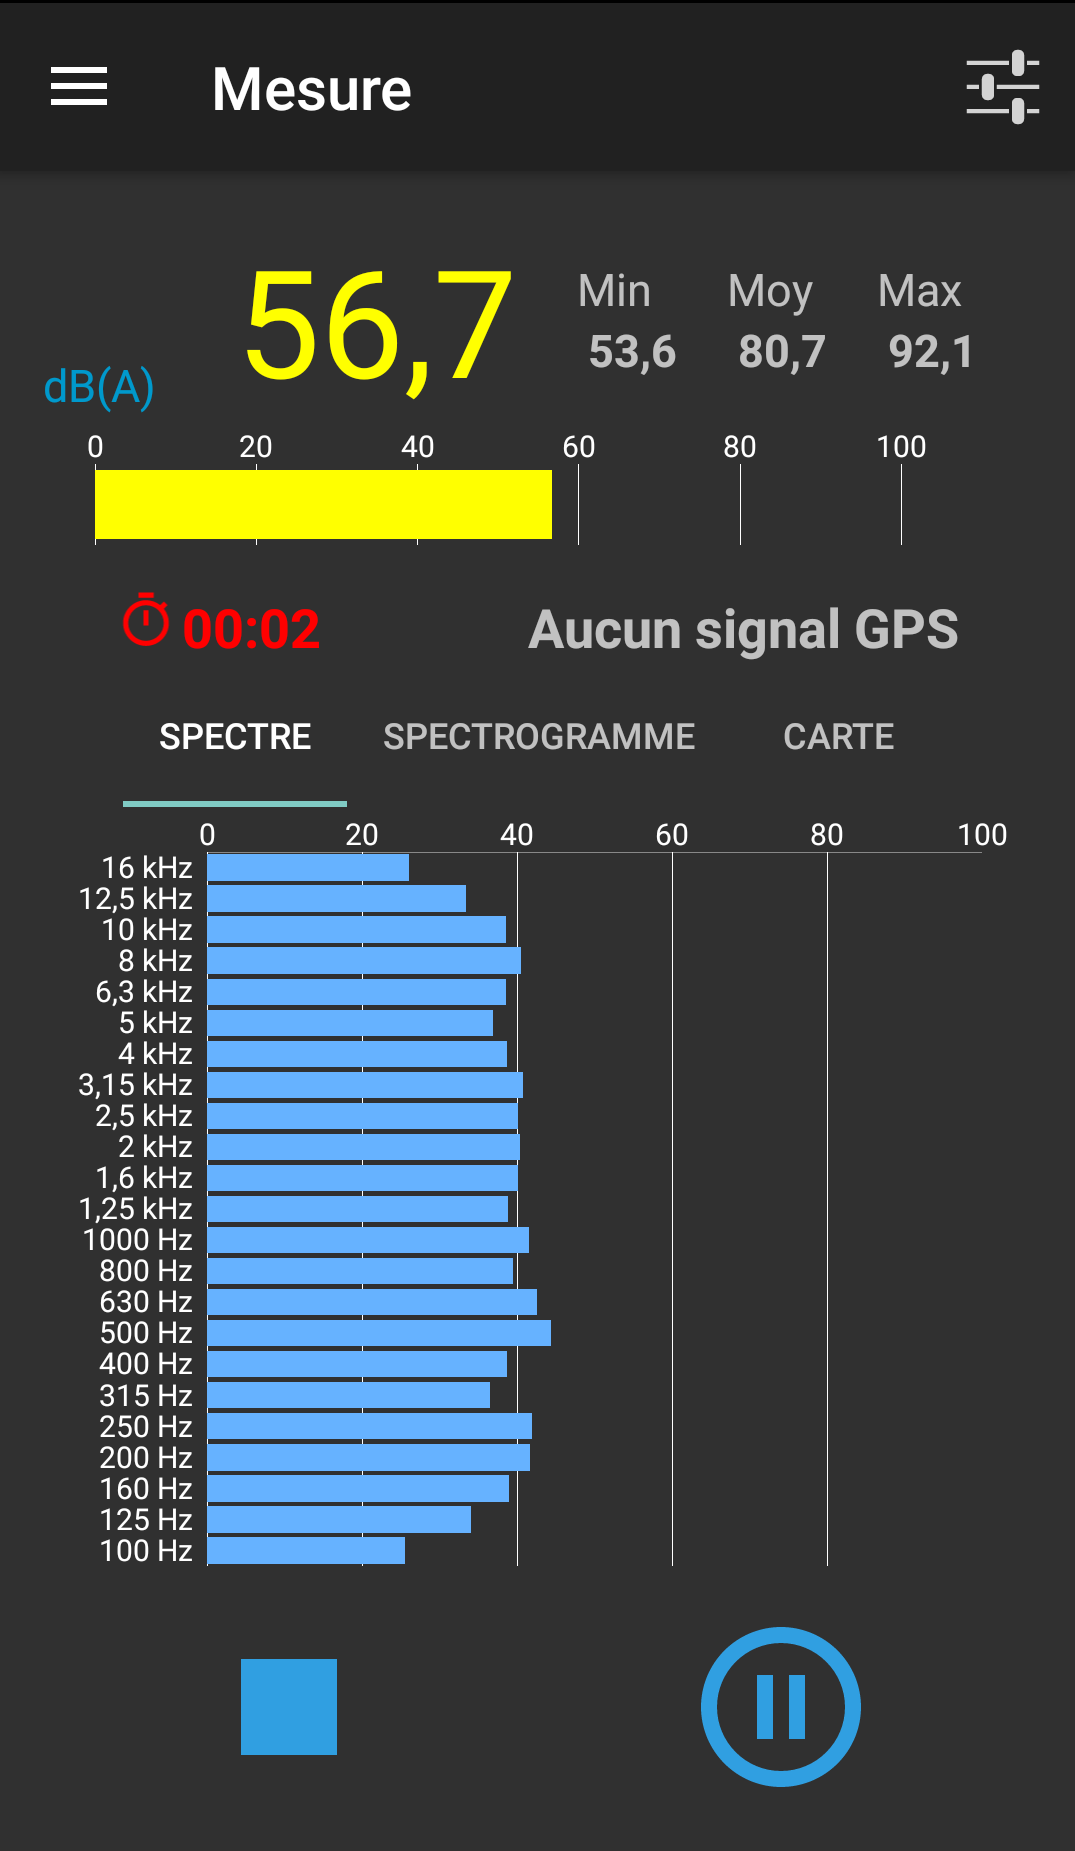
\includegraphics[width=0.9\textwidth]{./figures/autres/noiseCapture1.png}
    \end{minipage}
    \begin{minipage}[t]{0.3\textwidth}
        \centering
        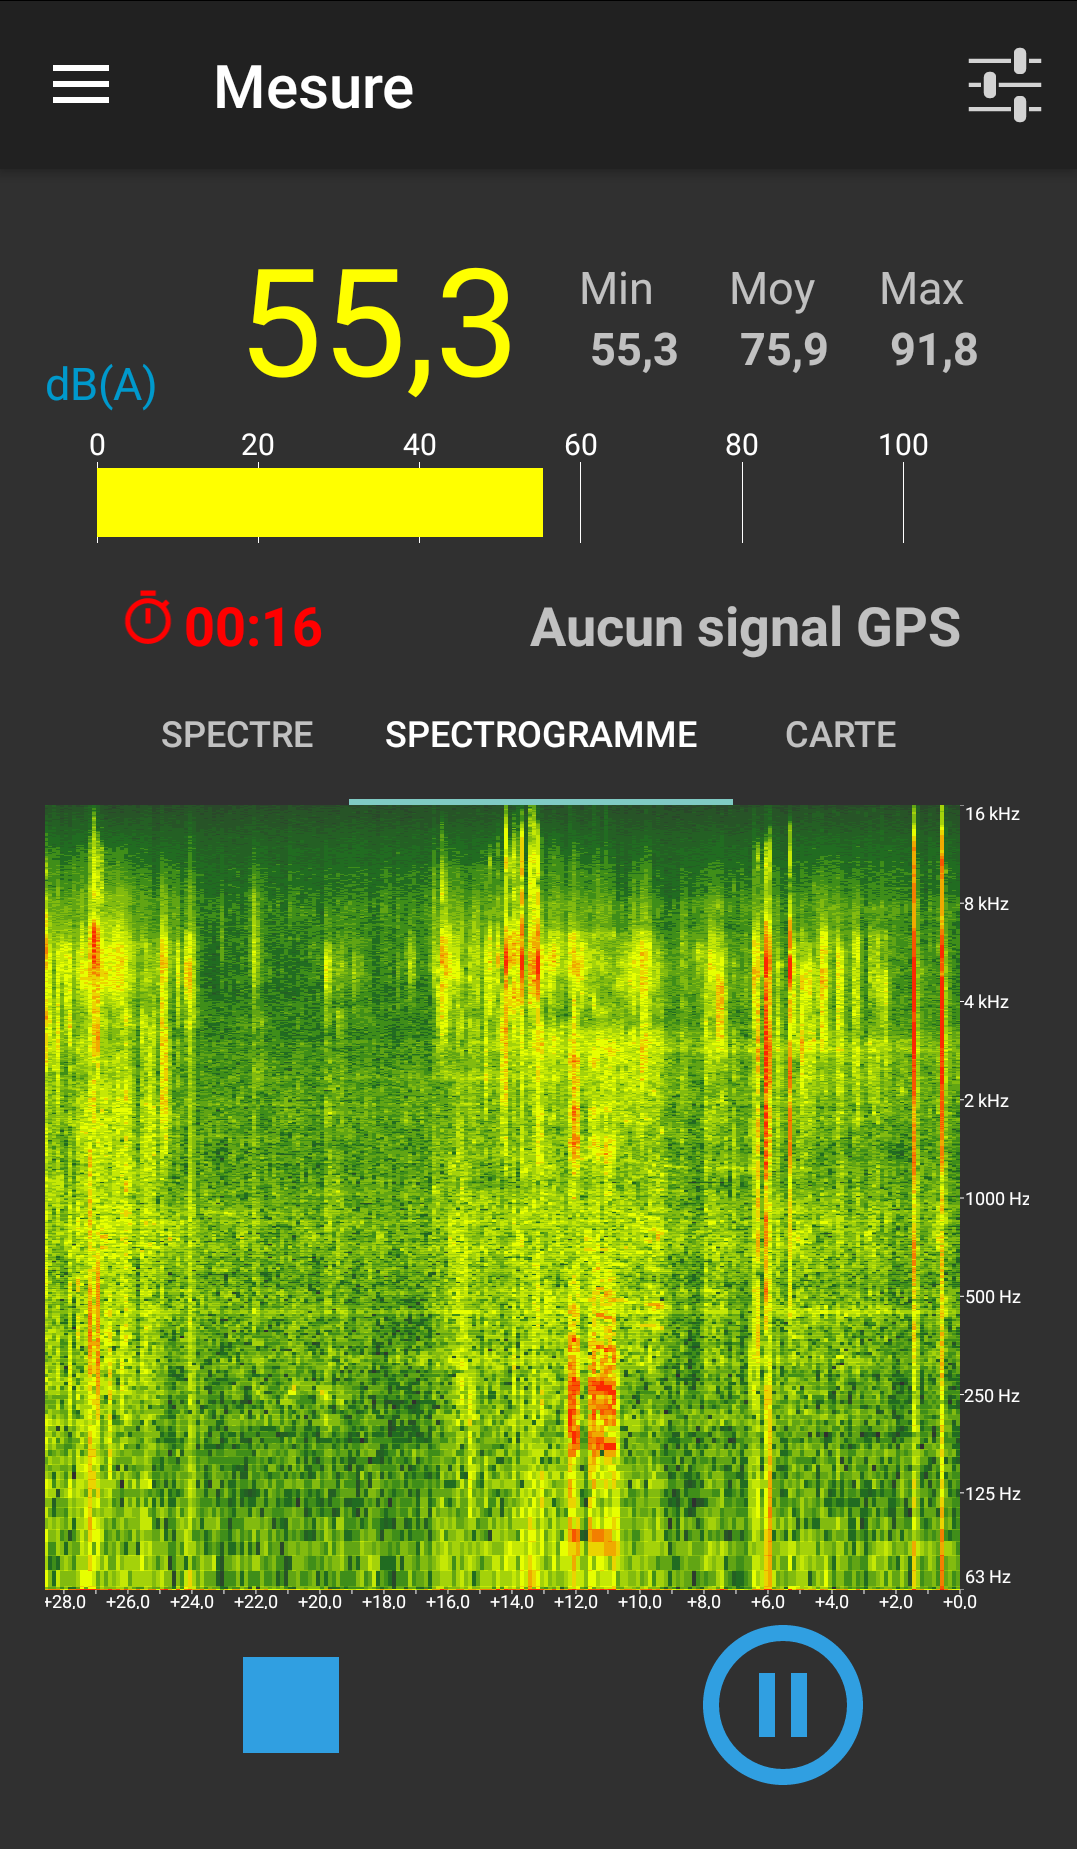
\includegraphics[width=0.9\textwidth]{./figures/autres/noiseCapture3.png}
    \end{minipage}
    \begin{minipage}[t]{0.3\textwidth}
        \centering
        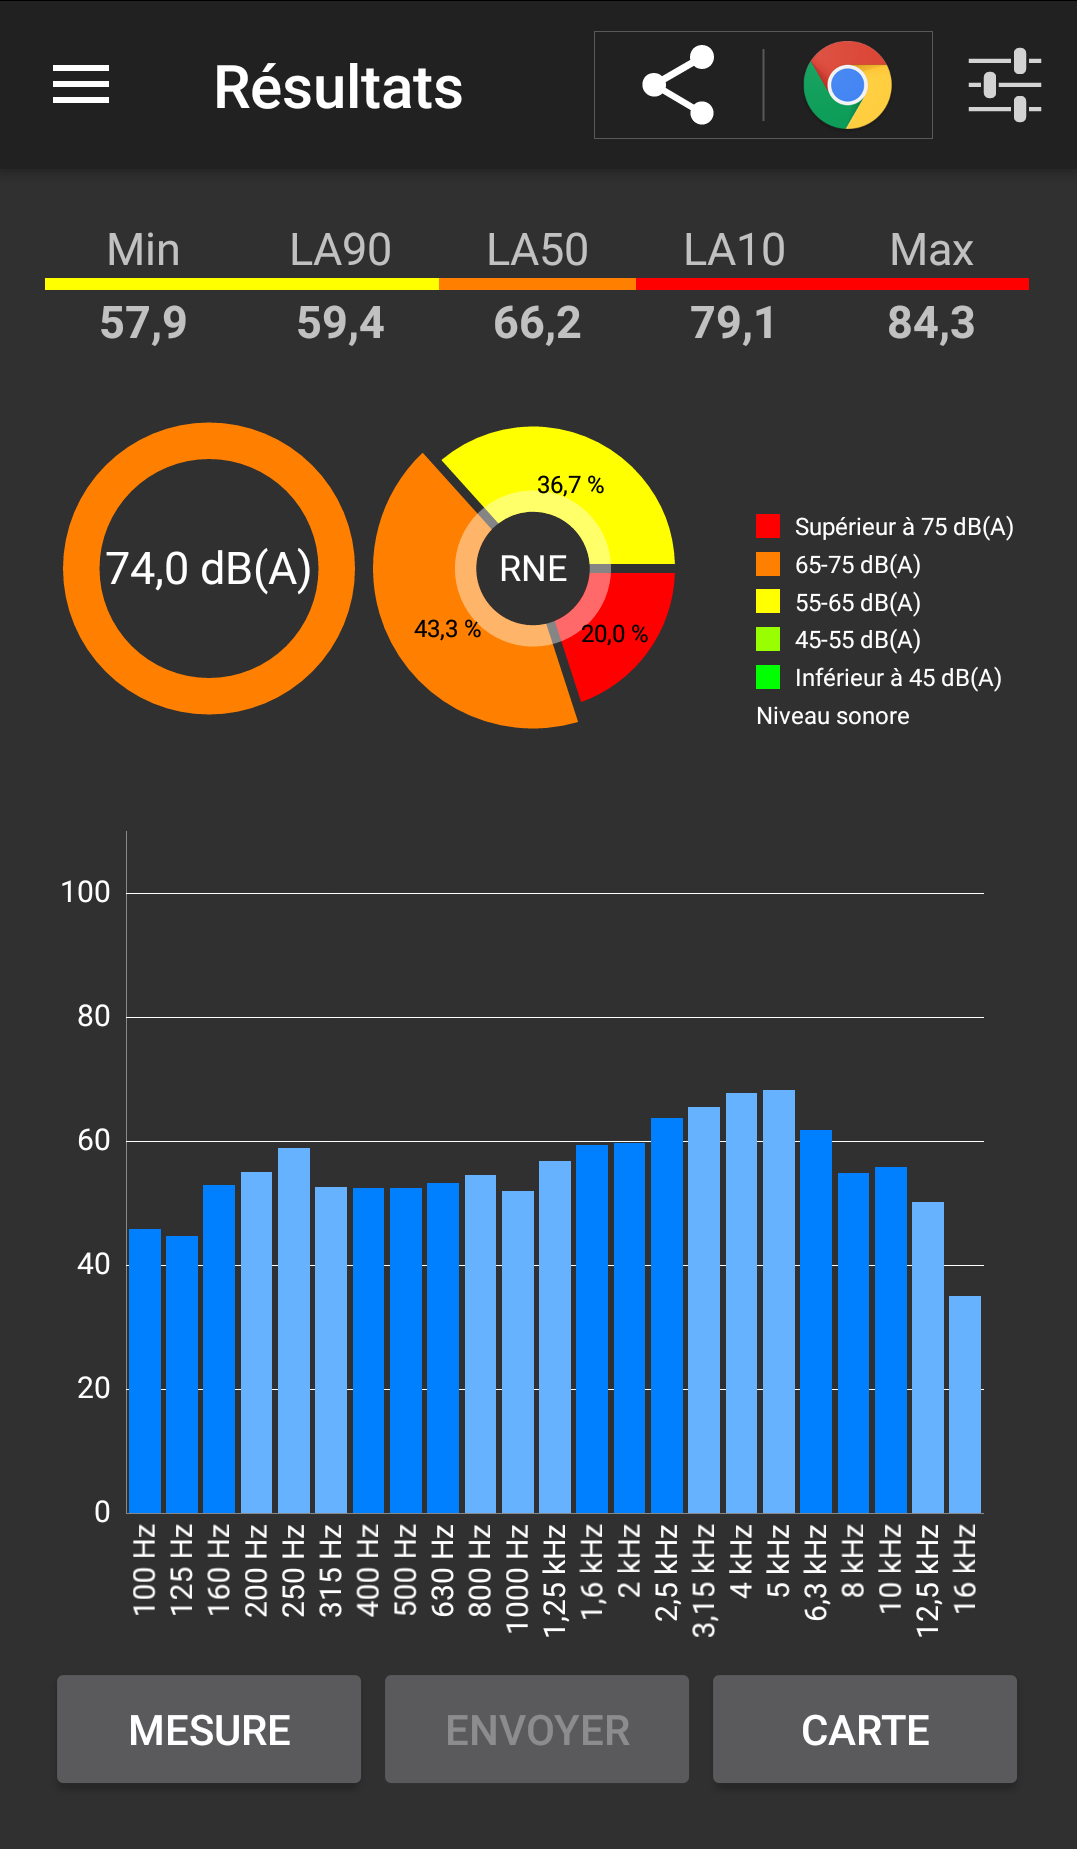
\includegraphics[width=0.9\textwidth]{./figures/autres/noiseCapture2.png}
    \end{minipage}
    \caption{Captures d'écran de l'application \textit{NoiseCapture}}
\end{center}
    \label{fig:noiseCapture}
\end{figure}

\subsection{Mesures participatives}

Une dernière voie sollicite la participation des citadins. Ces mesures participatives peuvent se réaliser en équipant les citadins de dispositifs spécifiques \cite{delaitre2014influence} ou bien à partir d'applications développées pour smartphones qu'ils peuvent télécharger eux-mêmes. Profitant de la démocratisation de ces appareils et de l'augmentation de leurs performances, ces applications leur permettent d'avoir un dispositif suffisamment performant pour mesurer les niveaux sonores autour d'eux. Cette approche permet surtout d'obtenir un plus grand nombre de mesures qui ont le plus souvent une distribution spatiale et temporelle plus aléatoire mais qui sont aussi effectuées moins régulièrement. L'utilisation de ces mesures est toutefois encore sujet à caution puisque de nombreux problèmes sont encore à résoudre comme la calibration et la prise en compte des performances des microphones dans les faibles et forts niveaux sonores \cite{aumond2017study} ou bien encore la qualité de la réalisation de la mesure faite par l'utilisateur\dots{} Dans ce cas, le traitement statistique des résultats est primordial afin de détecter les mesures incongrues et ne pas les considérer \cite{guillaume2016noise}. Plusieurs applications ont été dévelopées comme \textit{NoiseSpy} \cite{kanjo_noisespy_2010} ou \textit{Ambicity} \cite{ventura2017estimation}. On peut également relever dans le projet \textit{Noise Planet}\footnote{\url{http://noise-planet.org}} l'application pour smartphone, \textit{NoiseCapture} \cite{guillaume2016noise} (Figure \ref{fig:noiseCapture}), qui permet, là aussi, à l'utilisateur d'évaluer les niveaux sonores l'entourant tout en ayant la possibilité de décrire, à l'aide de mots-clés prédéfinis, les sons présents et l'ambiance sonore de la scène. La géo-localisation et les mesures sont ensuite collectées puis traitées pour produire des cartes de bruits, publiées en ligne (voir Figure \ref{fig:carte_noiseModelling}). Un des intérêts de ces applications, en plus de sensibiliser le citadin à son environnement sonore, est de le rendre producteur et utilisateur de données environnementales. Les informations récoltées sur ces trajets permettent de calculer son exposition au bruit ou bien de le guider vers des itinéraires secondaires où son exposition au bruit serait plus faible \cite{aumond2016sound}.\\

\begin{figure}[t]
\centering
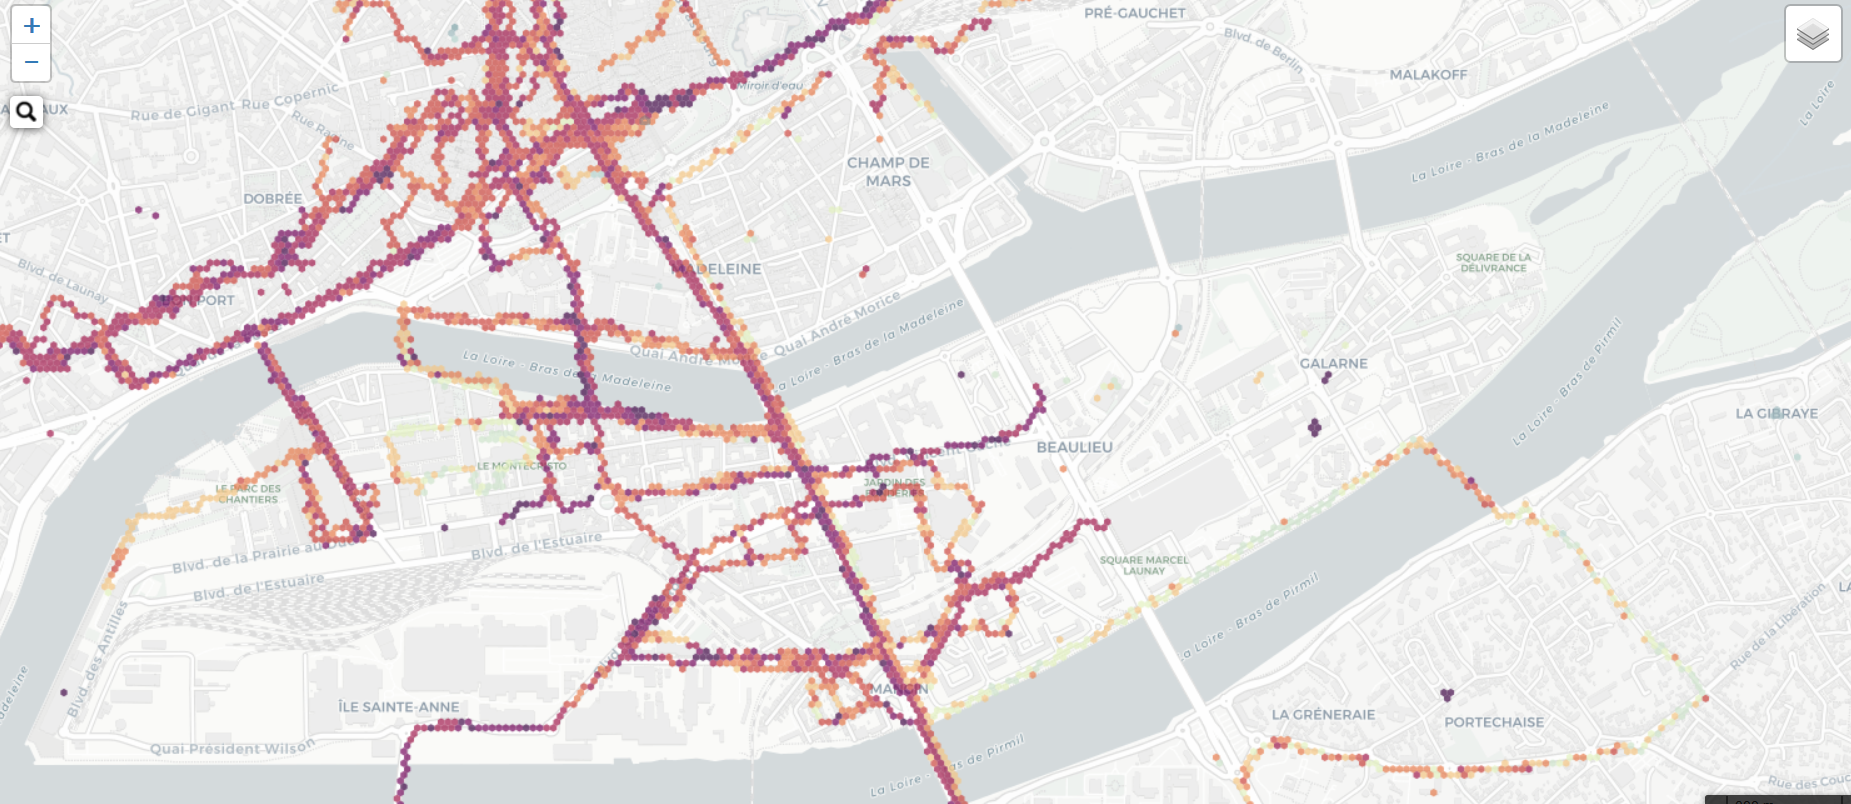
\includegraphics[width=0.7\linewidth]{./figures/cartographie/noise_modelling.PNG}
\caption{Carte de l'ESU de l'île de Nantes mesurée par l'application \textit{NoiseCapture}  (relevée le 22/03/2018)}
\label{fig:carte_noiseModelling}
\end{figure}

\subsection{Intérêts et limites des mesures faites en villes}

L'ensemble de ces dispositifs permet d'aborder l'ESU par une nouvel approche en s'affranchissant des problèmes liés à la modélisation des sources et de leur propagation dans l'environnement urbain et donnant plus facilement accès aux variations temporelles pour les réseaux de capteurs fixes. Ces méthodes ne sont toutefois pas exemptes de défauts. 
Dans le cas des réseaux de capteurs, leur installation et leur entretien a un coût important et sont des dispositifs lourd à gérer. De plus, la question de l'interpolation entre les points de mesures reste une source d'approximation. 
L'apport de mesures mobiles, à l'inverse, est de mieux estimer les variations spatiales aux dépends des variations à long-terme et peuvent être très couteuses en temps à réaliser à l'échelle d'une ville. Enfin les mesures participatives présentent des nombreuses incertitudes quant à la qualité de la mesure dues aux performances des capteurs des smartphones ou de la mesure réalisée qui nécessitent un traitement du signal important.

Mais malgré ces limites, en se basant sur des mesures \textit{in situ}, toutes sources confondues, ces dispositifs ouvrent la voies vers de nombreuses applications : 

\begin{itemize}
\item estimation des niveaux sonores du trafic et amélioration de la cartographie de bruit,
\item évaluation et classification plus complète des ESU au travers d'indicateurs physiques,
\item et représentation possible des ESU selon la perception des citadins.
\end{itemize}

Toutefois, en vue de prédire les niveaux de bruits du trafic ou de décrire les ESU selon les différentes sources sonores présentes, il est nécessaire de disposer d'outils de traitements  adaptés afin d'y extraire leur contributions. Hors, l'ESU est un milieu complexe, composé d'une multitude de sources variées (trafic routier, voix, oiseaux, klaxon, bruit de pas\dots) dont leurs allures temporelles (parfois brèves pour le retentissement d'un klaxon ou longues pour le passage d'une voiture) et fréquentielles (dans les basses fréquences pour le trafic, dans les hautes fréquences pour le sifflement des oiseaux) diffèrent, voir Figure \ref{fig:sourceUrbain}.
L'ensemble de ces sources est aussi susceptible d'être généré simultanément. La création d'outils adaptés à cet environnement pour reconnaitre ou détecter des sources spécifiques n'est donc pas triviale et a peu été traitée. Par exemple, dans le cas du trafic routier, s'il existe des endroits où celui-ci est prépondérant sur les autres sources sonores (périphérique, grand boulevard), il peut l'être moins dans d'autres lieux (dans des rues calmes, au niveau de parc) où ce sont d'autres sources sonores qui sont majoritairement présentes (voix, oiseaux \dots). En conséquence, ne pas isoler une source sonore spécifique parmi celles présentes risque de mener à de mauvaises estimations de leur temps de présence et de leur niveau sonore. \\

Il est donc nécessaire de générer un outil adapté à l'étude des mesures et enregistrements faits en villes pour y extraire les contributions et les niveaux sonores des sources présentes en villes. Cet aspect est une limite à l'utilisation de ces méthodes qu'il est nécessaire de résoudre afin de faciliter le déploiement de la mesure acoustique en ville.
En conséquence, les travaux de cette thèse cherchent à répondre à ces questions :

\begin{itemize}
\item \textbf{Comment déterminer le niveau sonore du trafic routier en ville ? est-il possible de déterminer ceux d'autres sources ?}
\item \textbf{Quelles sont les méthodes disponibles pour réaliser cette tâche ? Quel est l'outil le plus adapté à cet environnement parmi ces méthodes ?}
\item \textbf{Quel protocole expérimental mettre en place pour tester et valider les performances de cet outil ?}
\end{itemize}

\begin{figure}[t]
\centering
\subfigure[\label{fig:sourceUrb1}]{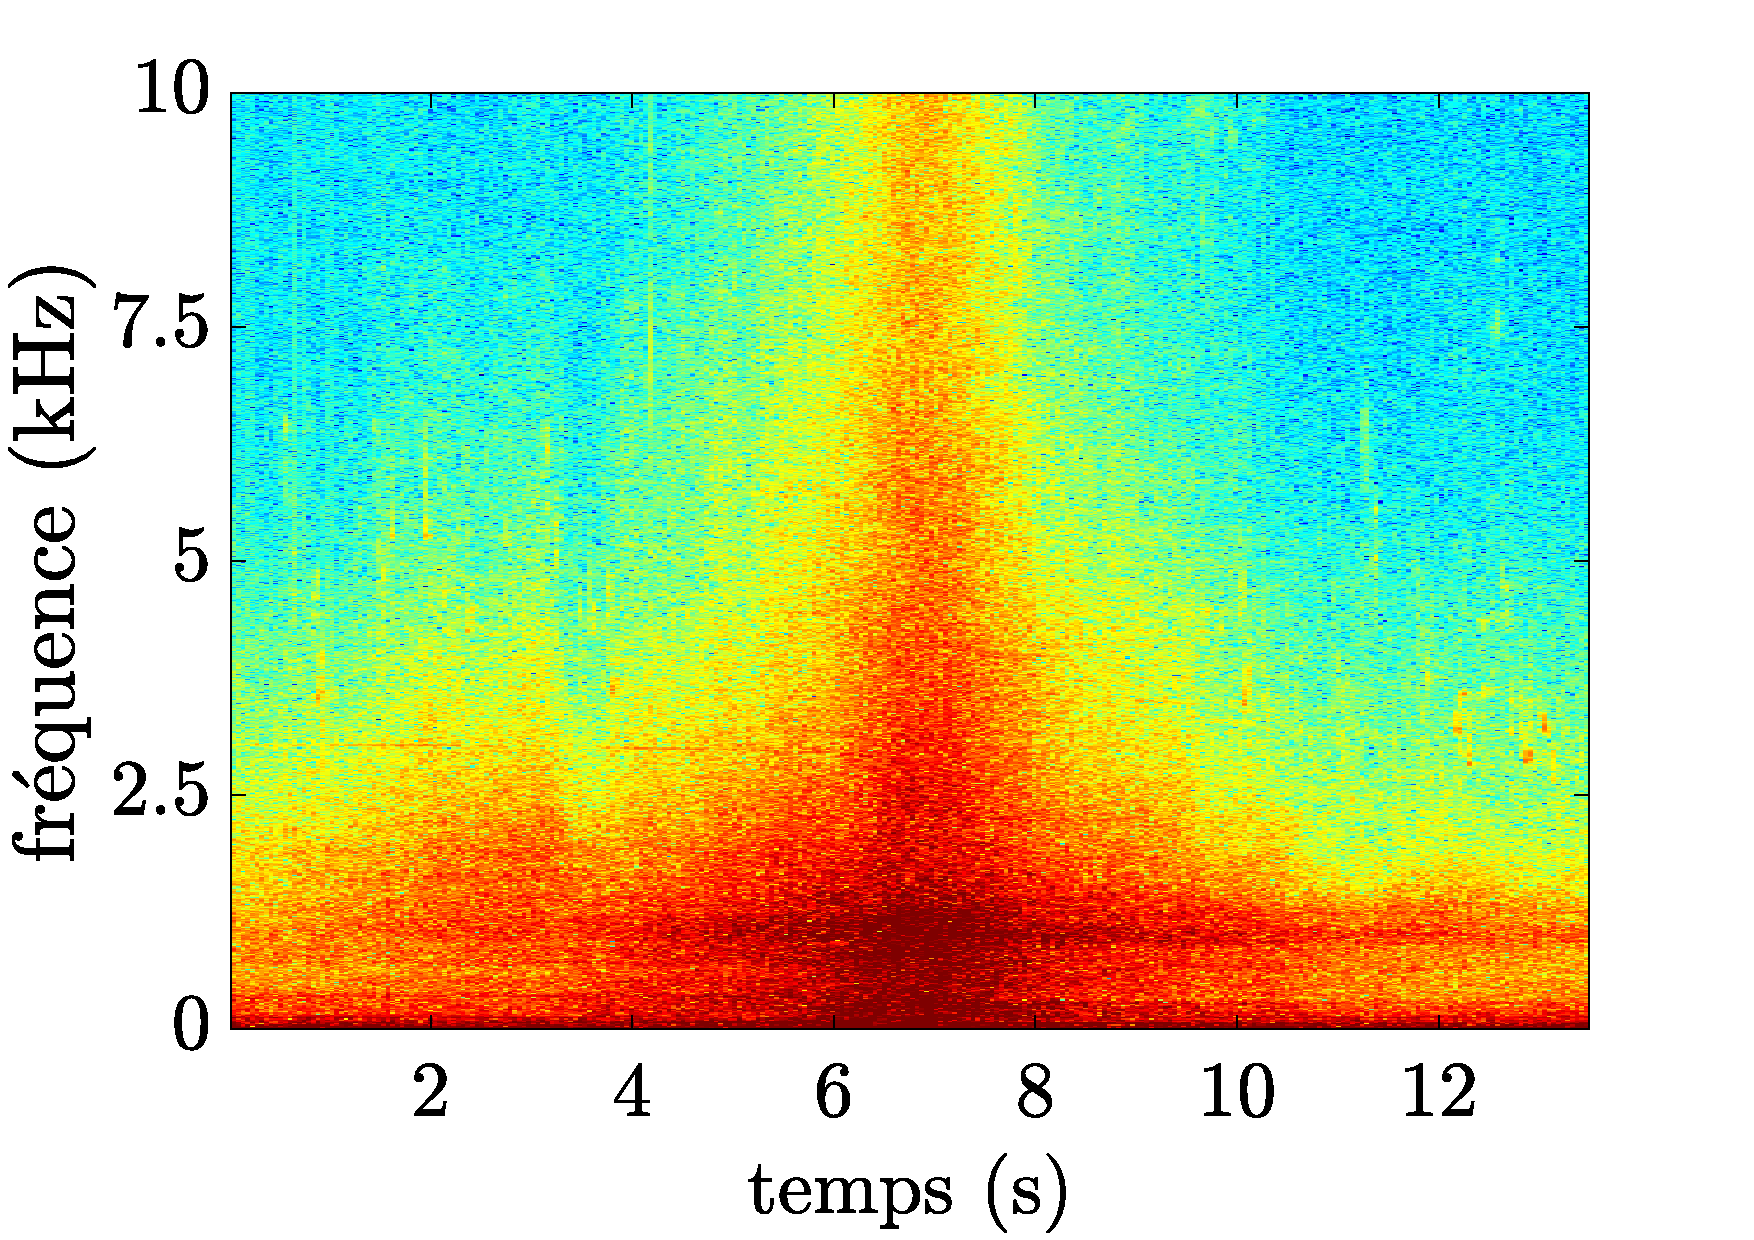
\includegraphics[width=0.4\linewidth]{./figures/autres/sourcesUrbainesCar.pdf}}
\subfigure[\label{fig:sourceUrb2}]{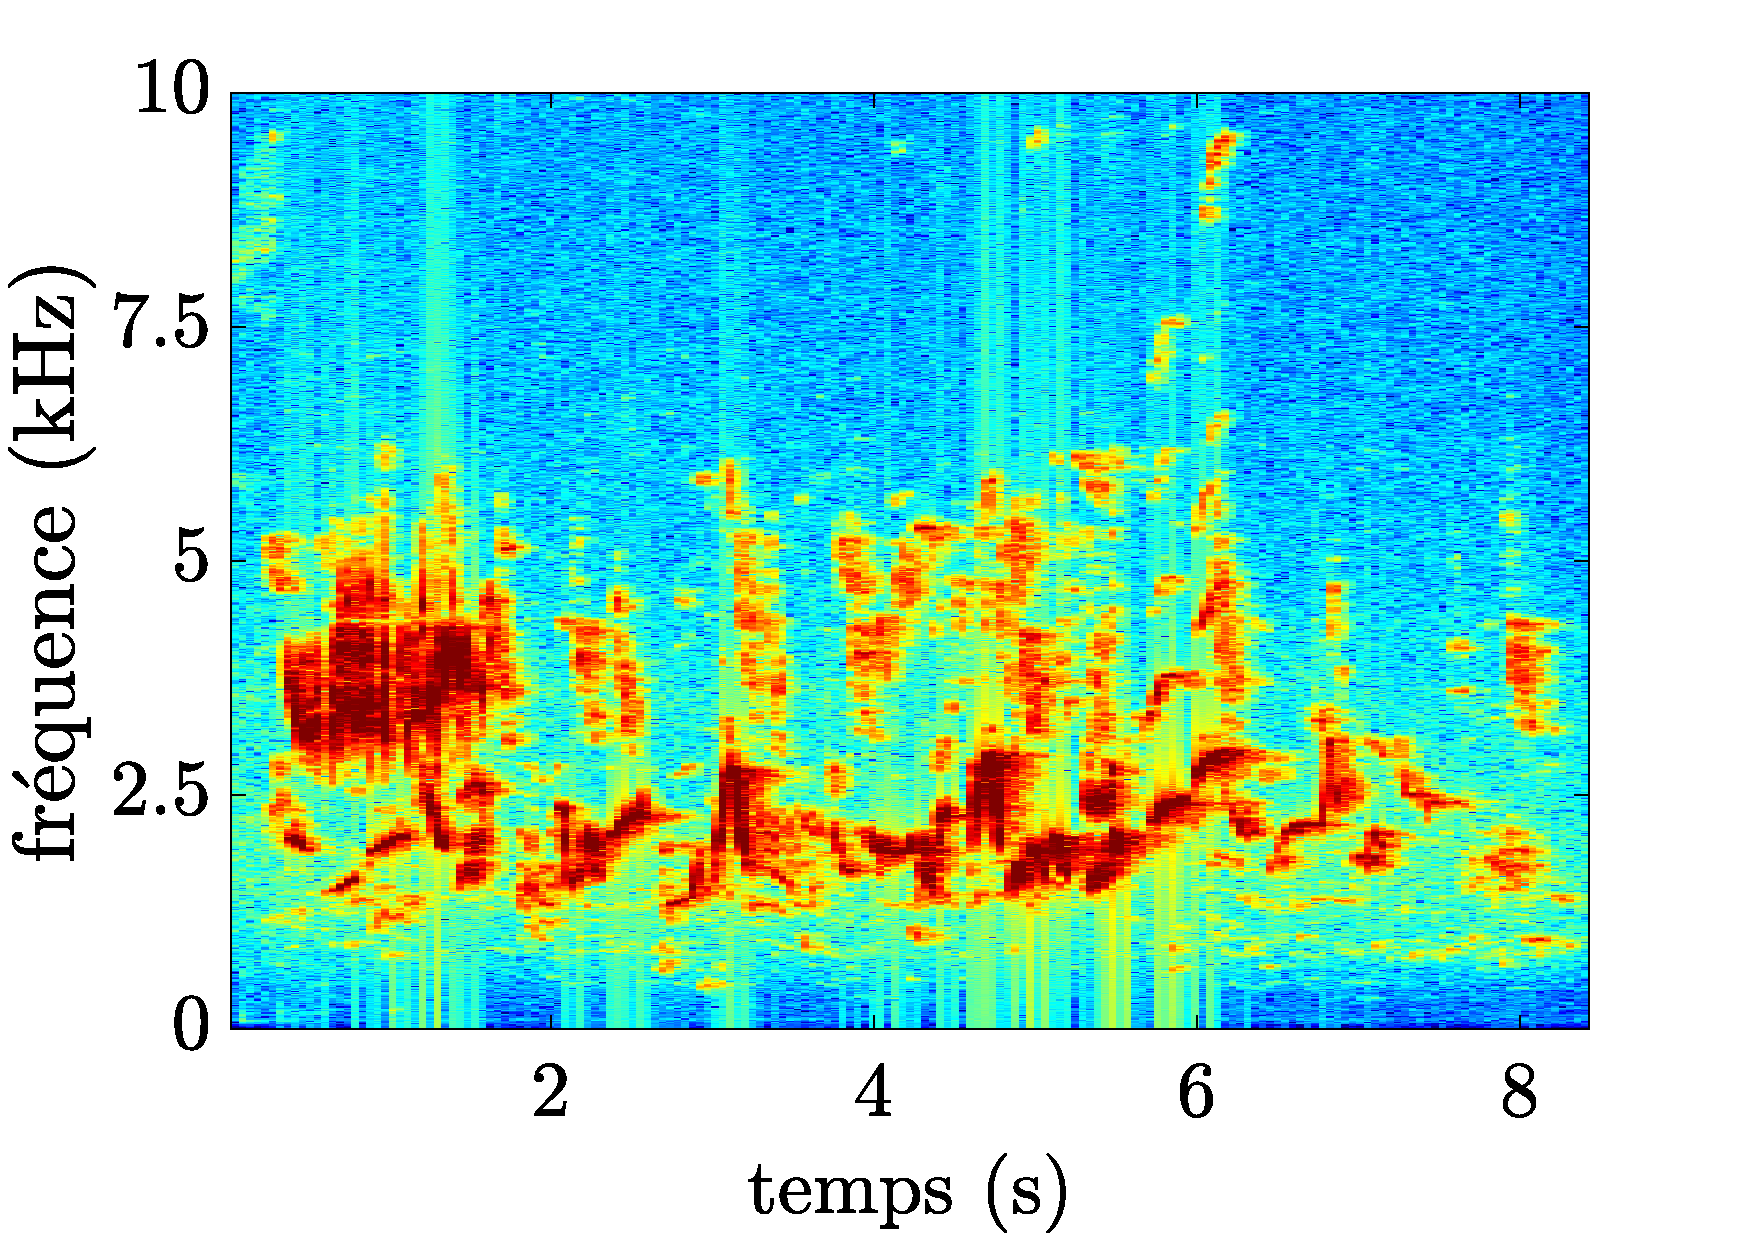
\includegraphics [width=0.4\linewidth]{./figures/autres/sourcesUrbainesBird.pdf}}
\subfigure[\label{fig:sourceUrb3}]{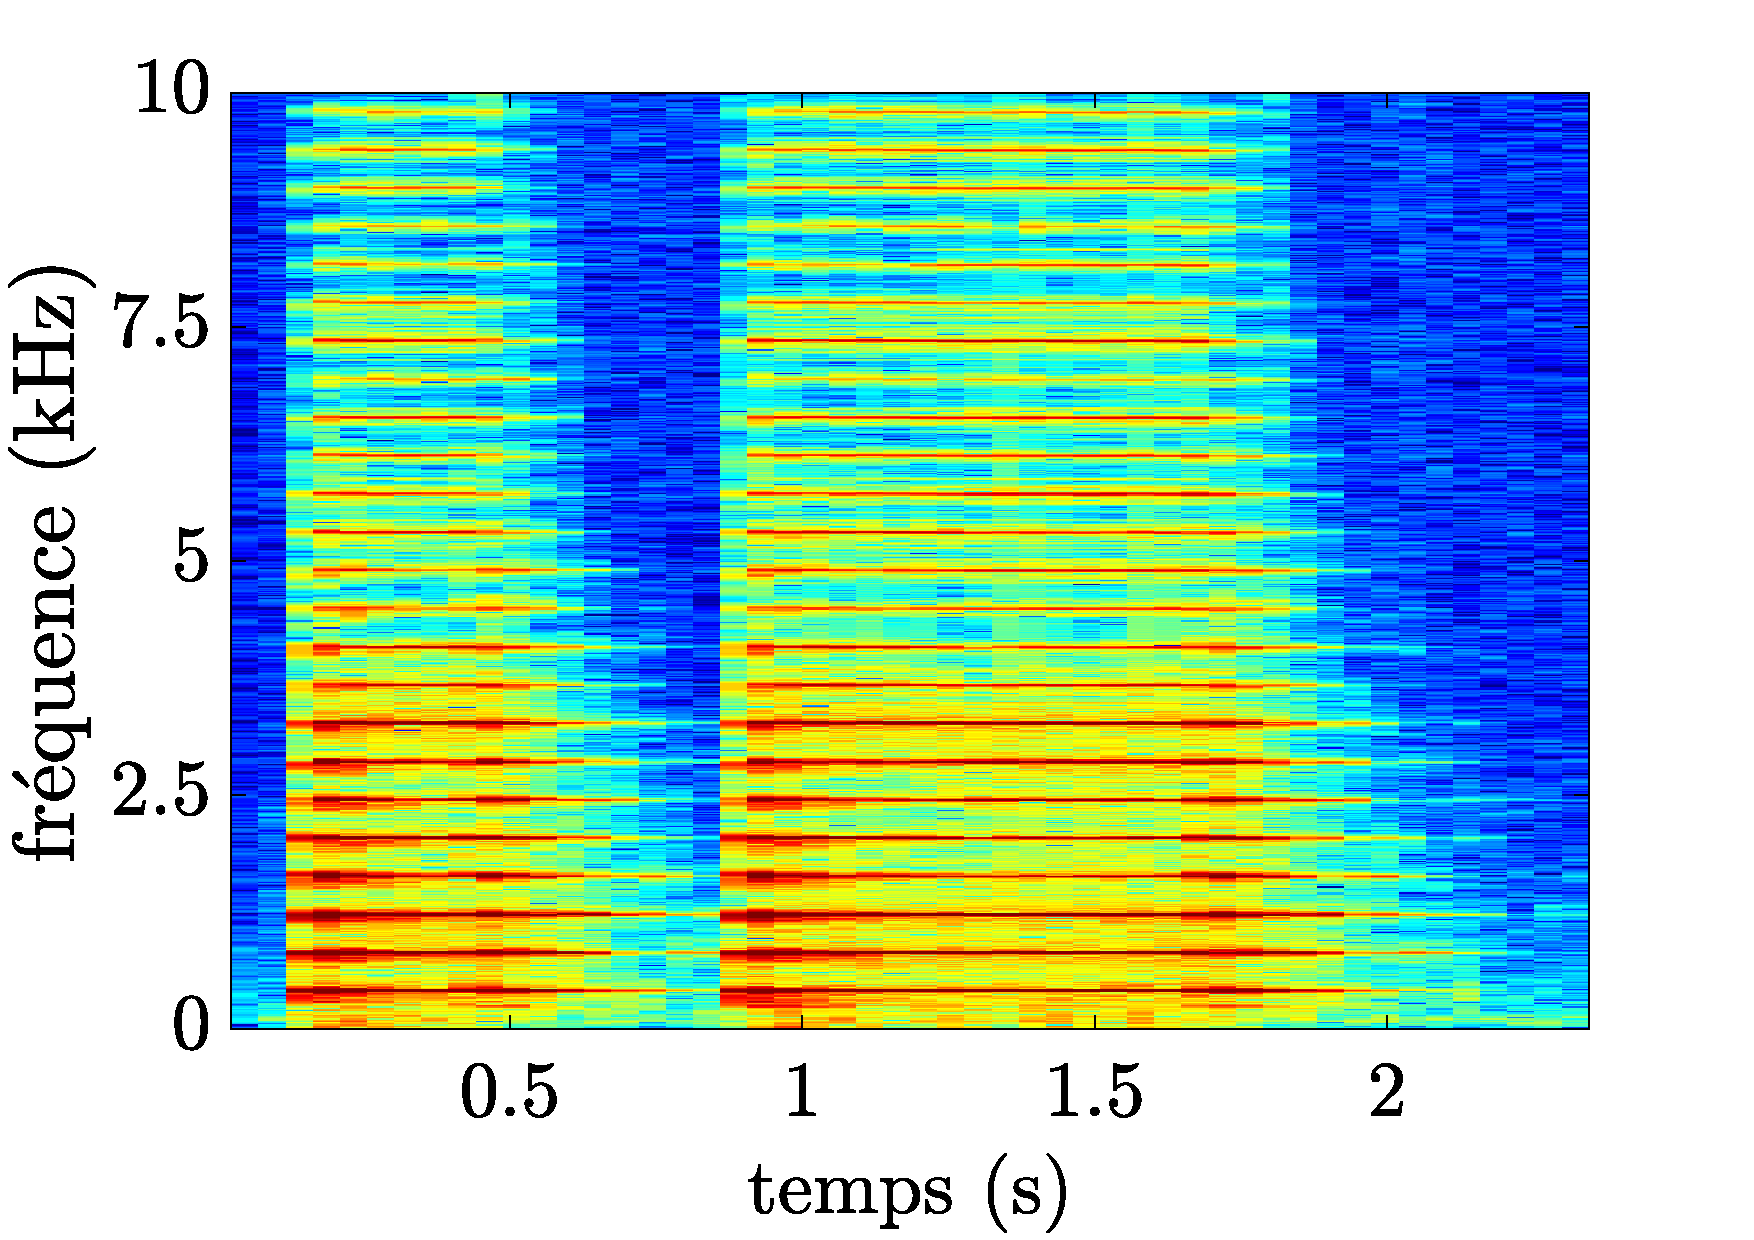
\includegraphics [width=0.4\linewidth]{./figures/autres/sourcesUrbainesCarHorn.pdf}}
\subfigure[\label{fig:sourceUrb4}]{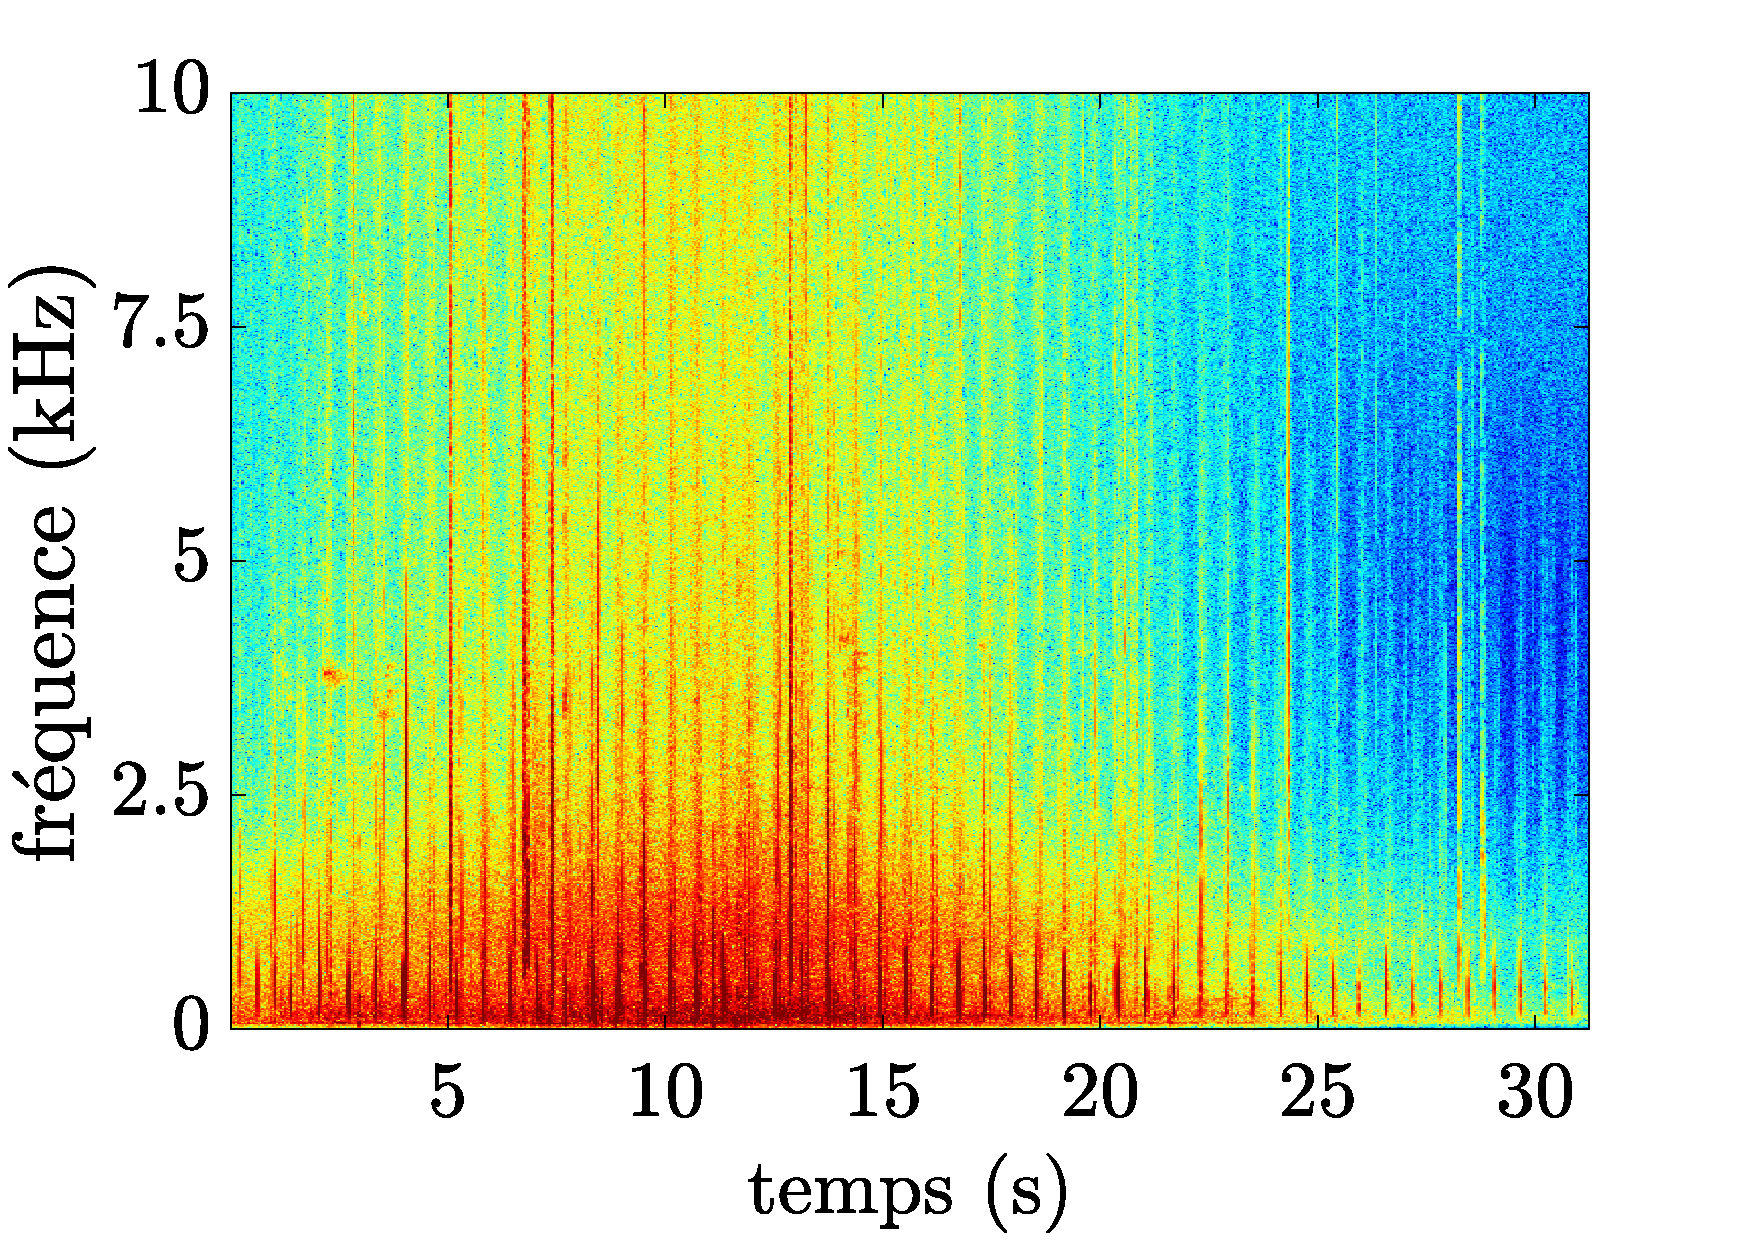
\includegraphics [width=0.4\linewidth]{./figures/autres/sourcesUrbainesFootStep.pdf}}
\caption{Spectrogrammes d'un passage d'une voiture \subref{fig:sourceUrb1}, d'un sifflement d'oiseaux \subref{fig:sourceUrb2}, d'un klaxon \subref{fig:sourceUrb3} et d'un bruit de pas \subref{fig:sourceUrb4}.}
\label{fig:sourceUrbain}
\end{figure}

\section{Estimation du niveau sonore du trafic routier} \label{part:cachier_charges}

Étant la source principale de bruit en ville ainsi que la plus gênante, le trafic routier sera la source d'intérêt qui sera principalement étudiée dans ce document. Le principe général de la méthode proposée est résumé en Figure \ref{fig:estimateur0} : à partir d'un enregistrement audio monophonique (réalisé en format wav et de fréquence d'échantillonnage 44,1 kHz), un outil, appelé \textit{estimateur}, détermine le niveau sonore estimé du trafic routier $\tilde{L}_{eq,trafic}$.
L'objectif est donc de construire cet estimateur et un protocole expérimental adéquat afin d'obtenir la meilleure estimation possible du niveau sonore du trafic.\\

\begin{figure}[ht]
\centering
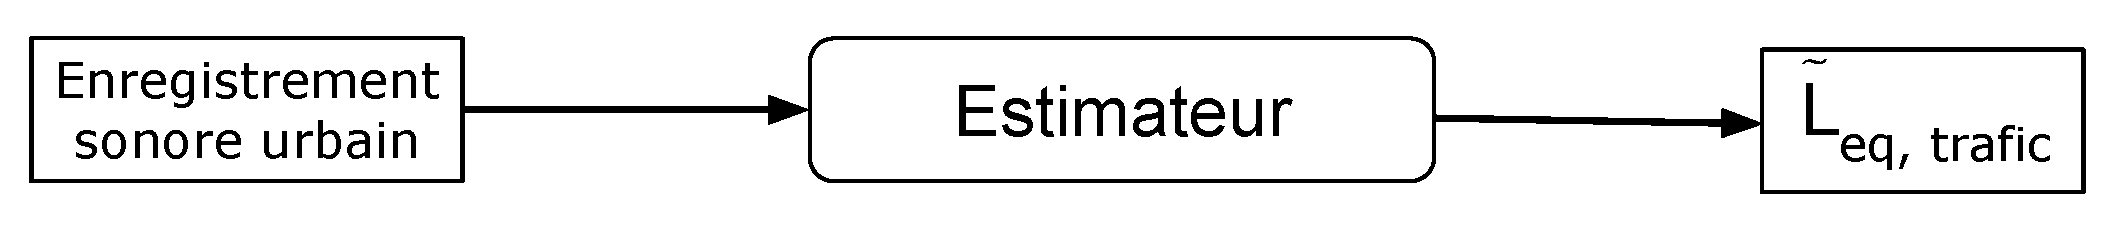
\includegraphics[width=0.7\linewidth]{./figures/NMF/bloc_diagram_estimateur0.pdf}
\caption{Vue synthétique de l'approche proposée.}
\label{fig:estimateur0}
\end{figure}


Parmi les travaux disponibles en littérature qui s'intéresse au trafic routier à partir d'enregistrements sonores d'ESU on trouve des outils de reconnaissance du bruit \cite{defreville_automatic_2006}, d'estimation du débit véhicule \cite{torija2012using}, de détection d'accidents de la route \cite{harlow2001automated} ou bien d'estimation des trajectoires \cite{leiba2017large} basé sur l'antennerie de microphones.
La détermination de son niveau sonore du trafic routier en tenant compte des autres sources sonores présentes parmi ces enregistrement a pour l'instant été très peu étudiée. On peut citer les travaux réalisés récemment au sein du projet DYNAMAP \cite{socoro2017anomalous}. Leur approche consiste à entrainer une méthode de détection en vue d'estimer les trames temporelles où la classe de son \textit{trafic} n'est pas présente afin de les rejeter lors de l'estimation des niveaux sonores. 

Ici, l'approche choisie est différente : l'estimateur du niveau sonore du trafic routier s'appuie sur une méthode de séparation de sources (voir chapitre \ref{chap:methode_separation_source}) afin d'extraire l'intégralité de la composante \textit{trafic} des enregistrements audio parmi les autres sources sonores présentes (voir Figure \ref{fig:separation_source}). De cette extraction, le niveau sonore trafic $\tilde{L}_{eq,trafic}$ est calculé.

\begin{figure}[ht]
\centering
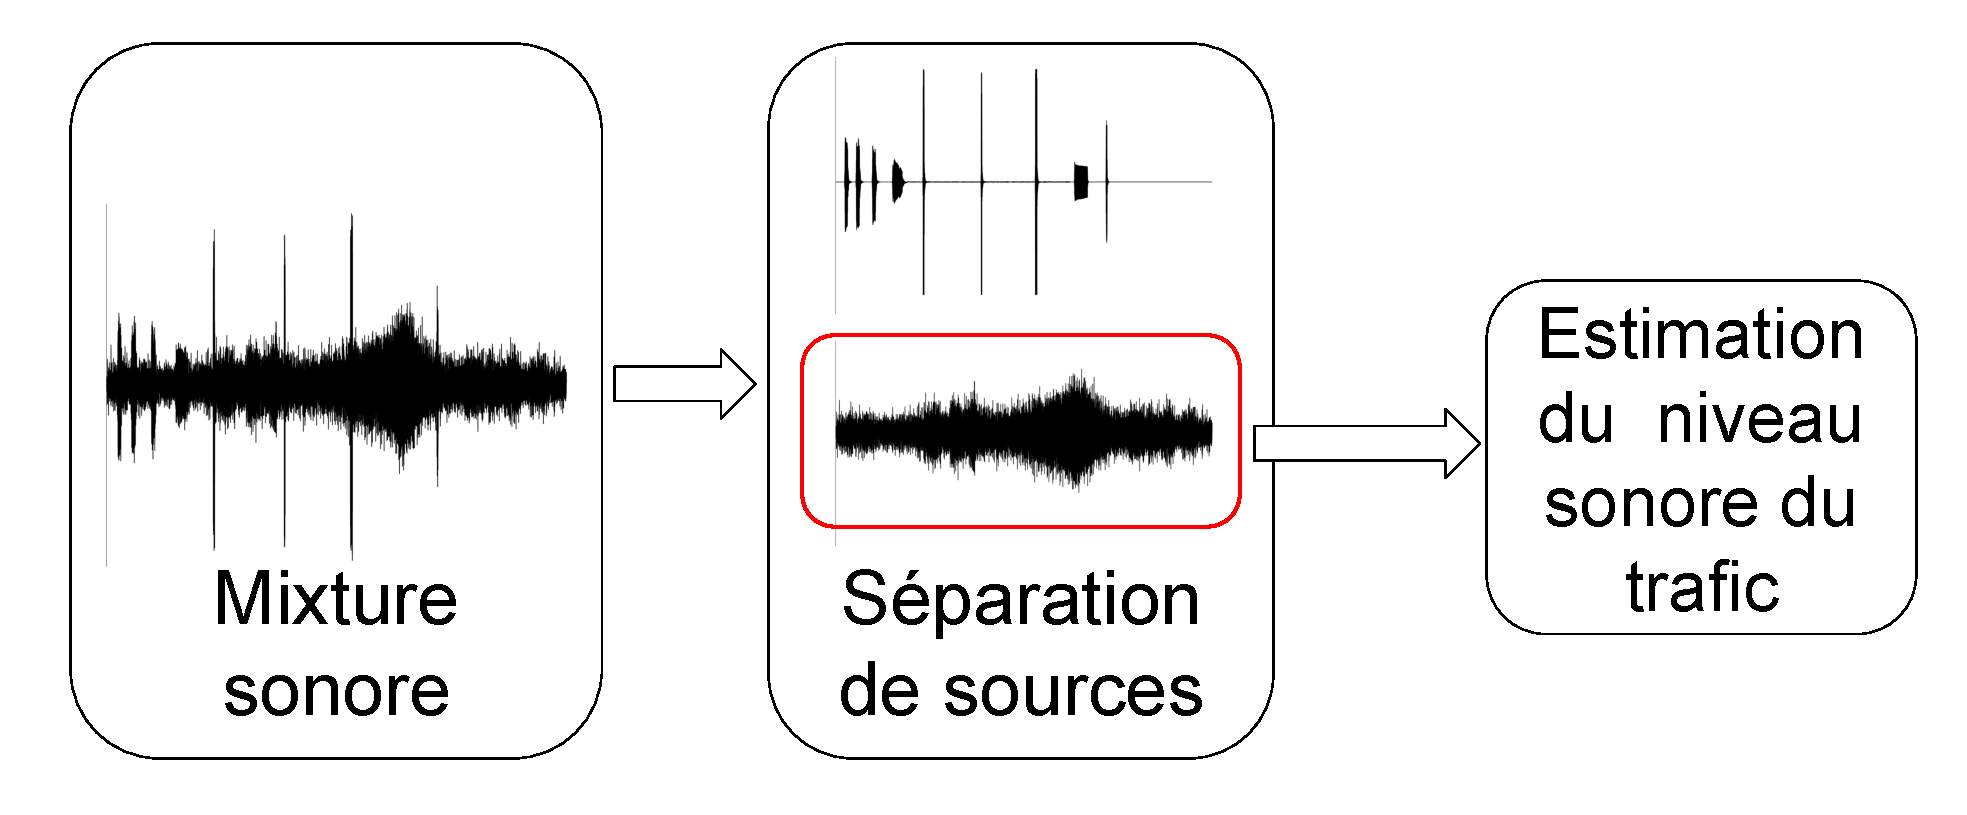
\includegraphics[width=0.7\linewidth]{./figures/NMF/bloc_diagram_source_separation.pdf}
\caption{Diagramme en bloc de l'approche par séparation de sources.}
\label{fig:separation_source}
\end{figure}

La comparaison de cette approche face aux travaux réalisés dans le projet DYNAMAP sera réalisée dans la partie \ref{part:comparaison_method}. Une question reste toutefois à résoudre : comment, à partir d'enregistrements audio, être certain que l'estimateur donne une valeur correcte du niveau sonore du trafic ? Dans le cas où il n'y a que du trafic, l'estimation fournie par la méthode peut être facilement comparée mais quid des scènes sonores où le trafic n'est pas prépondérant et est recouvert par d'autres sources sonores ? La valeur exacte du trafic, $L_{eq,trafic}$, est l'inconnue qu'on cherche justement à déterminer. Sans cette valeur de référence, il est impossible de comparer la valeur déterminée et ainsi la validité et les performances de l'estimateur.
Le choix est donc fait ici d'utiliser non pas des enregistrements sonores mais des corpus de scènes sonores issus d'un processus de simulation où un contrôle complet des classes sonores présentes, ainsi que de leur niveau sonore, est alors possible. Grâce à ce procédé, la valeur exacte, $L_{eq,trafic}$, peut ainsi être alors obtenue. La Figure \ref{fig:diagramBlocProtocol} résume le schéma global du procédé suivi.

\begin{figure}[ht]
\centering
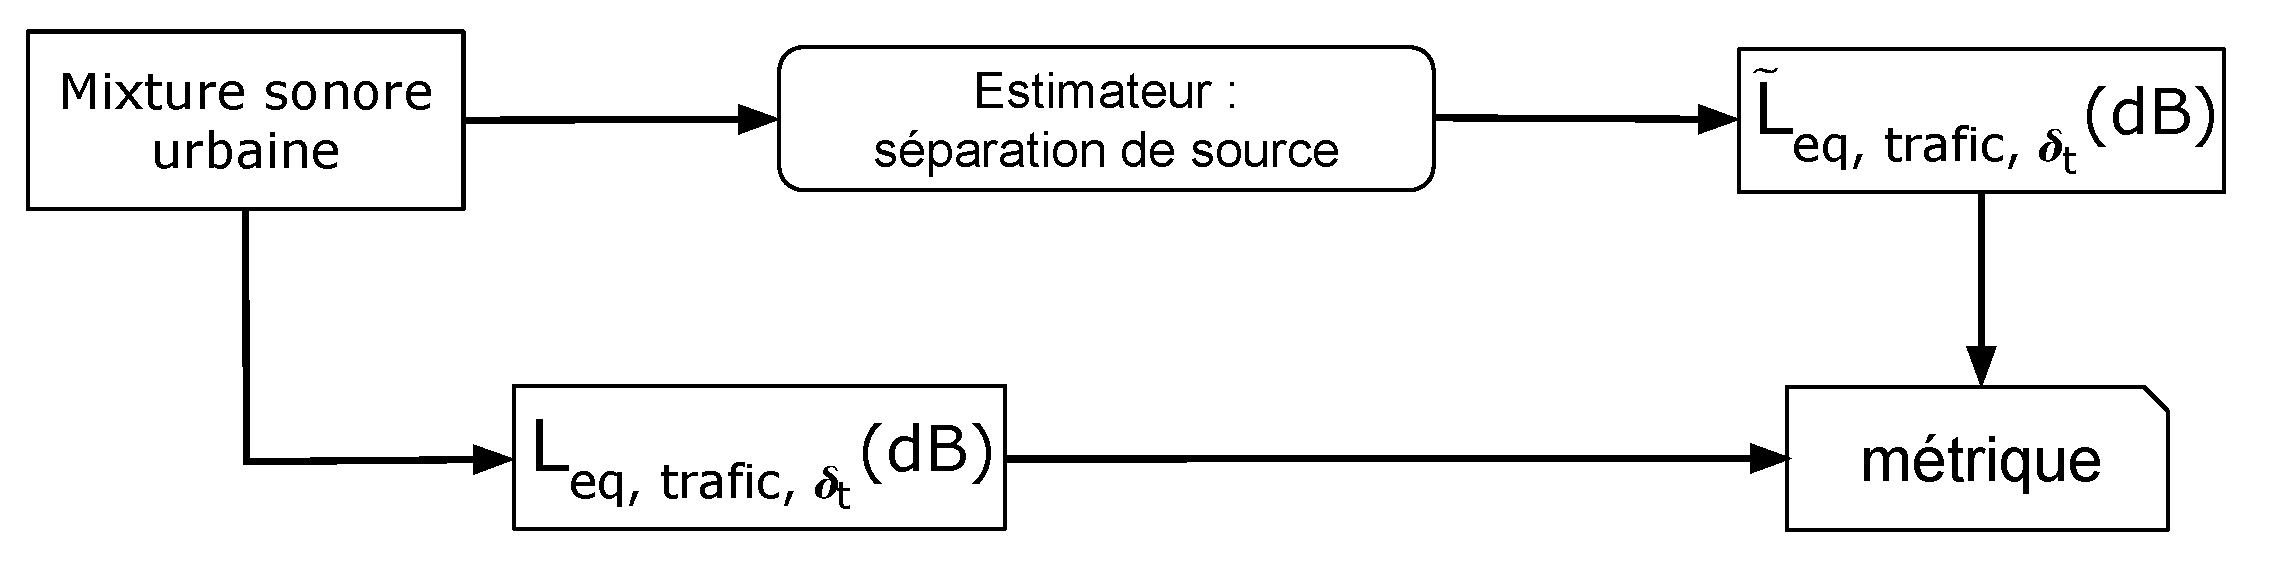
\includegraphics[width=0.7\linewidth]{./figures/NMF/Bloc_diagram_estimateur_FR.pdf}
\caption{Diagramme bloc du protocole expérimental.}
\label{fig:diagramBlocProtocol}
\end{figure}

Se pose alors la question du niveau sonore calculé par scène : choisit-on un niveau sonore à court-terme toutes les 125 ms ? toutes les secondes ? toutes les minutes ? pondéré $A$ ? Aux vues de l'utilisation de cet estimateur qui est faite (meilleur estimation de la contribution du trafic, amélioration de la cartographie des cartes de bruits en ville), le choix est fait de ne considérer aucune pondération afin de se focaliser sur une estimation physique du niveau \textit{trafic} ainsi que de choisir une durée d'intégration $\delta_t$ longue pour le calcul des niveaux sonores. 
Dans un premier temps, sur le premier corpus (voir partie \ref{part:corpus_ambiance}), la durée des scènes étant la même (30 secondes), le temps d'intégration sera alors de 30 secondes ($L_{eq,trafic,30s}$). Puis, dans un second corpus (partie \ref{part:corpus_grafic}), la durée des scènes sonores étant variable, on choisira un temps d'intégration à la minute ($L_{eq,trafic,60s}$).\\

Les niveaux sonores exacts et estimés, produits sur un ensemble de $M$ scènes testés, sont ensuite comparés à travers un calcul de métrique. Parmi les différentes métriques possibles (somme des carrés des résidus, la racine de l'erreur quadratique moyenne $RMSE$ \dots), l'erreur absolue moyenne, $MAE$ (pour \textit{Mean Absolute Error}) est retenue :

\begin{equation}
MAE = \frac{\sum_{i = 1}^{M} \vert L_{eq, trafic, \delta t}^i - \tilde{L}_{eq, trafic, \delta t}^i \vert}{M}.
\end{equation}

Contrairement à l'erreur RMSE, qui revient à la racine carré de la moyenne du carré des différences entre les données observées et réelles, qui pénalise plus les valeurs qui dévie fortement, l'erreur $MAE$ présente l'intérêt de considérer un poids identique entre chaque différence et ainsi de gagner en interprétabilité.\\

À partir de cette proposition, il faut maintenant : 
\begin{itemize}
\item \textbf{déterminer quelle méthode de séparation de sources choisir comme estimateur, }
\item \textbf{construire correctement des corpus de scènes sonores urbaines pour tester l'efficacité de l'estimateur retenu.}
\end{itemize}



%
%%\bibliographystyle{unsrt}
%%\bibliography{../bibliographie}
%%
%%\end{document}

%
%Dans le domaine fréquentiel, le produit de convolution s'exprime sous la forme : 
%
%\begin{equation}
%\hat{M}_{i}(f) = \hat{s}_j(f)\hat{\delta}_{ij}(f)e^{i2\pi f \tau_{ij}} 
%\end{equation}
%
%avec $\hat{g}(f)$, la transformée de Fourier de la fonction $g(t)$, $\hat{g}(f) = \frac{1}{\sqrt{2\pi}}\int_{-\infty}^{+\infty}g(t)e^{-i2\pi ft} dt$. $\hat{\delta}_{ij}(f)$ s'apparente alors à un filtre de propagation.